% % \section{Использованные функции}

% % \begin{lstlisting}[caption={Функция для отображения исходного и преобразованного изображений}]
% % # show the source image and transformed image
% % def show_images(source, transformed, title="Image"):
% %     img_src_rgb = cv2.cvtColor(source, cv2.COLOR_BGR2RGB) # normal colors to display
% %     img_trf_rgb = cv2.cvtColor(transformed, cv2.COLOR_BGR2RGB) 

% %     plt.figure(figsize=(13, 5))
% %     plt.suptitle(title, fontsize=16)

% %     plt.subplot(1, 2, 1)
% %     plt.imshow(img_src_rgb)
% %     plt.title('Source Image')
% %     plt.text(10, 10, f'Resolution: {source.shape[1]}x{source.shape[0]}', color='white', backgroundcolor='black', fontsize=8, ha='left', va='top')
% %     plt.axis('off')

% %     plt.subplot(1, 2, 2)
% %     plt.imshow(img_trf_rgb)
% %     plt.title('Transformed Image')
% %     plt.text(10, 10, f'Resolution: {transformed.shape[1]}x{transformed.shape[0]}', color='white', backgroundcolor='black', fontsize=8, ha='left', va='top')
% %     plt.axis('off')

% %     # adjust space between images
% %     plt.subplots_adjust(wspace=0.3, hspace=0.3)
% %     plt.subplots_adjust(left=0.05, right=0.95)

% %     # save image
% %     plt.savefig(f"results/{title}.png")
% % \end{lstlisting}

% % \begin{lstlisting}[caption={Функция для применения матричных преобразований}]
% % def apply_matrix_transformations(img, matrix, shape=(0, 0)):
% %     # apply the matrix to the image
% %     if shape == (0, 0):
% %         shape = (img.shape[1], img.shape[0])
% %     return cv2.warpAffine(img, matrix, shape)
% % \end{lstlisting}

% % \begin{lstlisting}[caption={Функция для применения проективных преобразований}]
% % def apply_perspective_transformations(img, matrix, shape=(0, 0)):
% %     # apply the matrix to the image
% %     if shape == (0, 0):
% %         shape = (img.shape[1], img.shape[0])
% %     return cv2.warpPerspective(img, matrix, shape)
% % \end{lstlisting}

% % \begin{lstlisting}[caption={Функция для коррекции дисторсии}]
% % def distortion_correction(img, map_func):
% %     xi, yi = np.meshgrid(np.arange(img.shape[1]), np.arange(img.shape[0]))

% %     # shift and normalize grid 
% %     xmid, xmid = img.shape[1] / 2.0, img.shape[0] / 2.0
% %     xi = xi - xmid
% %     yi = yi - xmid

% %     # convert to polar coordinates
% %     r, theta = cv2.cartToPolar(xi / xmid, yi / xmid)
% %     r = map_func(r)

% %     # convert back to cartesian coordinates
% %     u, v = cv2.polarToCart(r, theta)

% %     u, v = u * xmid + xmid, v * xmid + xmid

% %     # remap the image
% %     return cv2.remap(img, u.astype(np.float32), v.astype(np.float32), cv2.INTER_LINEAR)
% % \end{lstlisting}

\href{https://github.com/edelwiw/TechVision_Lab2}{Исходный код на GitHub}. 

\section{Теоретическая часть}

Геометрические преобразования подразумевают пространственное изменение положения 
пикселей изображения, при этом интенсивность пикселей остается неизменной.

В двумерных плоских геометрических преобразованиях, как правило, используется декартова система координат.
В таком случае, перемещение пикселей на изображении можно описать с помощью матрицы преобразования.

Для общности с дальнейшими преобразованиями, будем использовать \textit{однородные координаты}.

Размерность однородного пространства равна $n - 1$, где $n$ -- количество координат.
Точка в однородном пространстве определяется как набор элементов $\left(x_0:x_1:\ldots:x_n\right)$, при этом хотя бы одни из элементов не должен быть равен 0. 
Кроме того, две точки в проективном пространстве считаются равными, если одну можно получить умножением другой на скаляр: $\left(x_1:x_2:\ldots:x_n\right)=\left(\lambda x_1:\lambda x_2:\ldots:\lambda x_n\right)$. То есть разные наборы координат могут задавать одну и ту же точку.   

\subsection{Матрица преобразования в однородной системе координат}

Матрица преобразования в такой системе координат выглядит следующим образом:

\begin{equation}
    T = \begin{bmatrix}
        A & B & C \\
        D & E & F \\
        G & H & I
    \end{bmatrix}
\end{equation}

{
\renewcommand*{\arraystretch}{0.4}
Коэффициенты $\left[\begin{matrix}A&B\\D&E\\\end{matrix}\right]$ из этой матрицы задают стандартное преобразование плоскости в декартовой системе координат, например, поворот относительно центра координат, масштабирование плоскости, центральная симметрия. 
Коэффициенты $\left[\begin{matrix}C\\F\\\end{matrix}\right]$ – коэффициенты перемещения в направлениях $x$ и $y$ соответственно. 
Коэффициенты  $\left[\begin{matrix}G&H\\\end{matrix}\right]$ отвечают за геометрическое проецирование. 
Последний коэффициент I\ отвечает за масштабирование. 
}

Для получения преобразованого изображения необходимо умножить матрицу преобразования на матрицу координат изображения:
\begin{equation}
    X' = T \times X
\end{equation}

\begin{figure}[ht]
    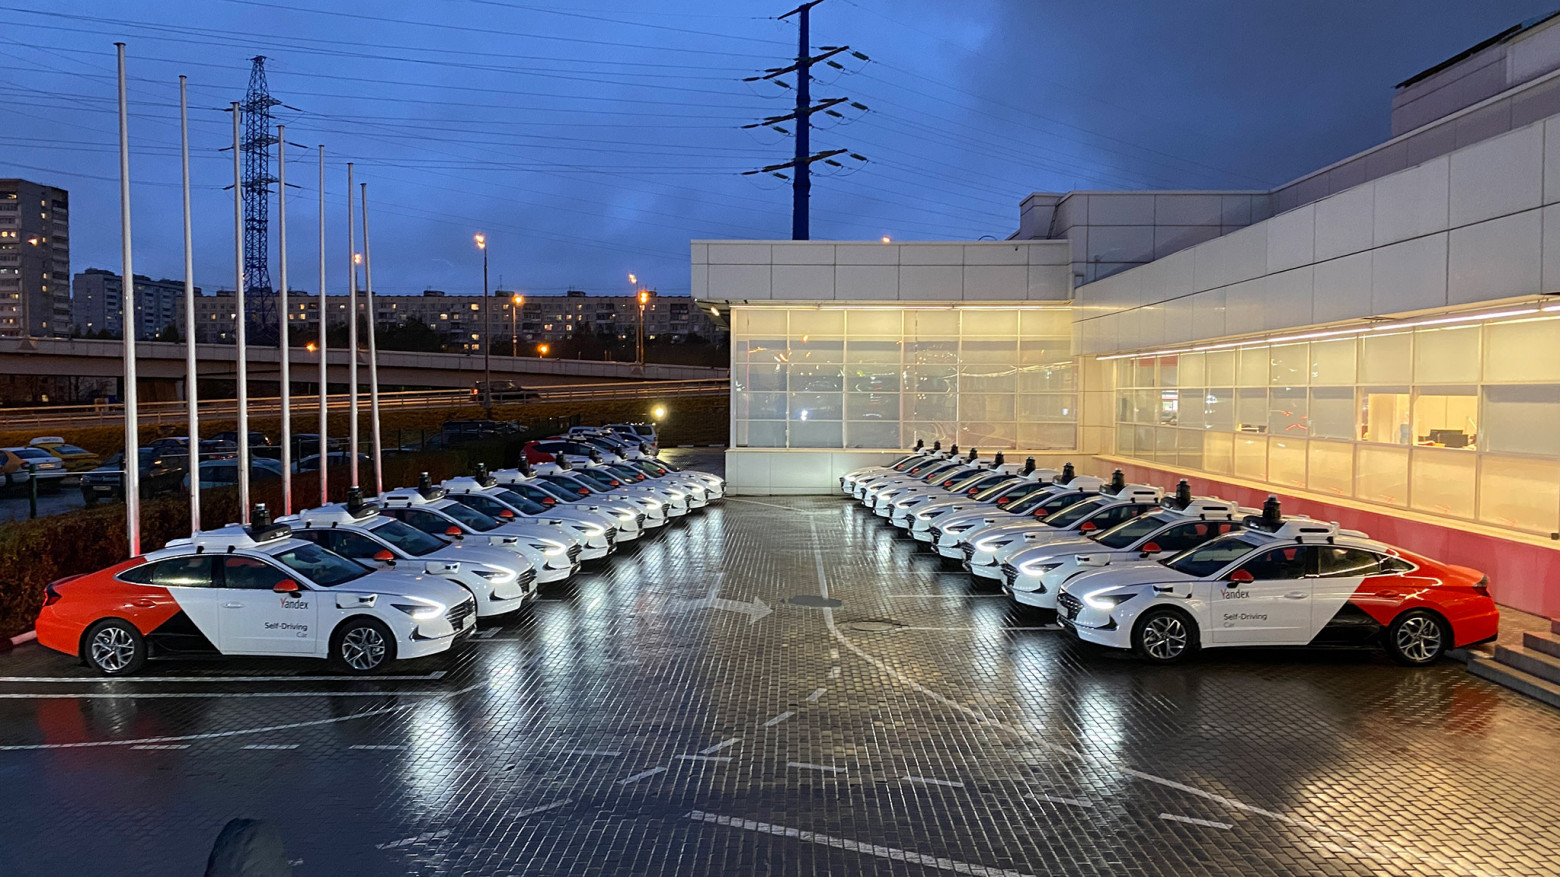
\includegraphics[width=\textwidth]{../source/image.png}
    \caption{Исходное изображение}
    \label{fig:source_image}
\end{figure}

\section{Линейные преобразования}

\textbf{Линейное отображение} -- такое отображение, при котором сохраняется форма бесконечно малых фигур и углы между прямыми в точках их пересечения. 
Эти преобразования являются частным случаем \textit{аффинных преобразований}.

\subsection{Сдвиг изображения}

Для того, чтобы сдвинуть изображение на вектор $(dx, dy)$, необходимо умножить координаты каждой точки изображения на матрицу преобразования:
\begin{equation}
    T = \begin{bmatrix}
        1 & 0 & dx \\
        0 & 1 & dy \\
        0 & 0 & 1
    \end{bmatrix}
\end{equation}
Соответственно, преобразованное изображение $I'$ можно получить следующим образом:
\begin{equation}
    X' = T \times X
\end{equation}
Рассмотрим как применить сдвиг на 150 пикселей вправо и 100 пикселей вниз к изображению:

\begin{lstlisting}[style=cpp_white, caption={Исходный код для сдвига изображения}]
T = (cv::Mat_<double>(2, 3) << 
                    1, 0, 150, 
                    0, 1, 100); 
cv::warpAffine(image, image_shift, T, cv::Size(image.cols, image.rows));

cv::imwrite(path + "/lab2/outputs/image_shift.png", image_shift);

cv::imshow("Shift image", image_shift); 
\end{lstlisting}

Для удобства отладки и сборки используется средство автоматизации сборки ПО:
\begin{lstlisting}[style=cpp_white, caption={CMakeLists.txt для сборки проекта}]
cmake_minimum_required(VERSION 2.8)

project( CV-lab2 )
find_package( OpenCV REQUIRED )

include_directories( ${OpenCV_INCLUDE_DIRS} )
add_executable( ${PROJECT_NAME}  src/lab2.cpp )

target_link_libraries( ${PROJECT_NAME} ${OpenCV_LIBS} )
\end{lstlisting}

\begin{figure}[ht]
    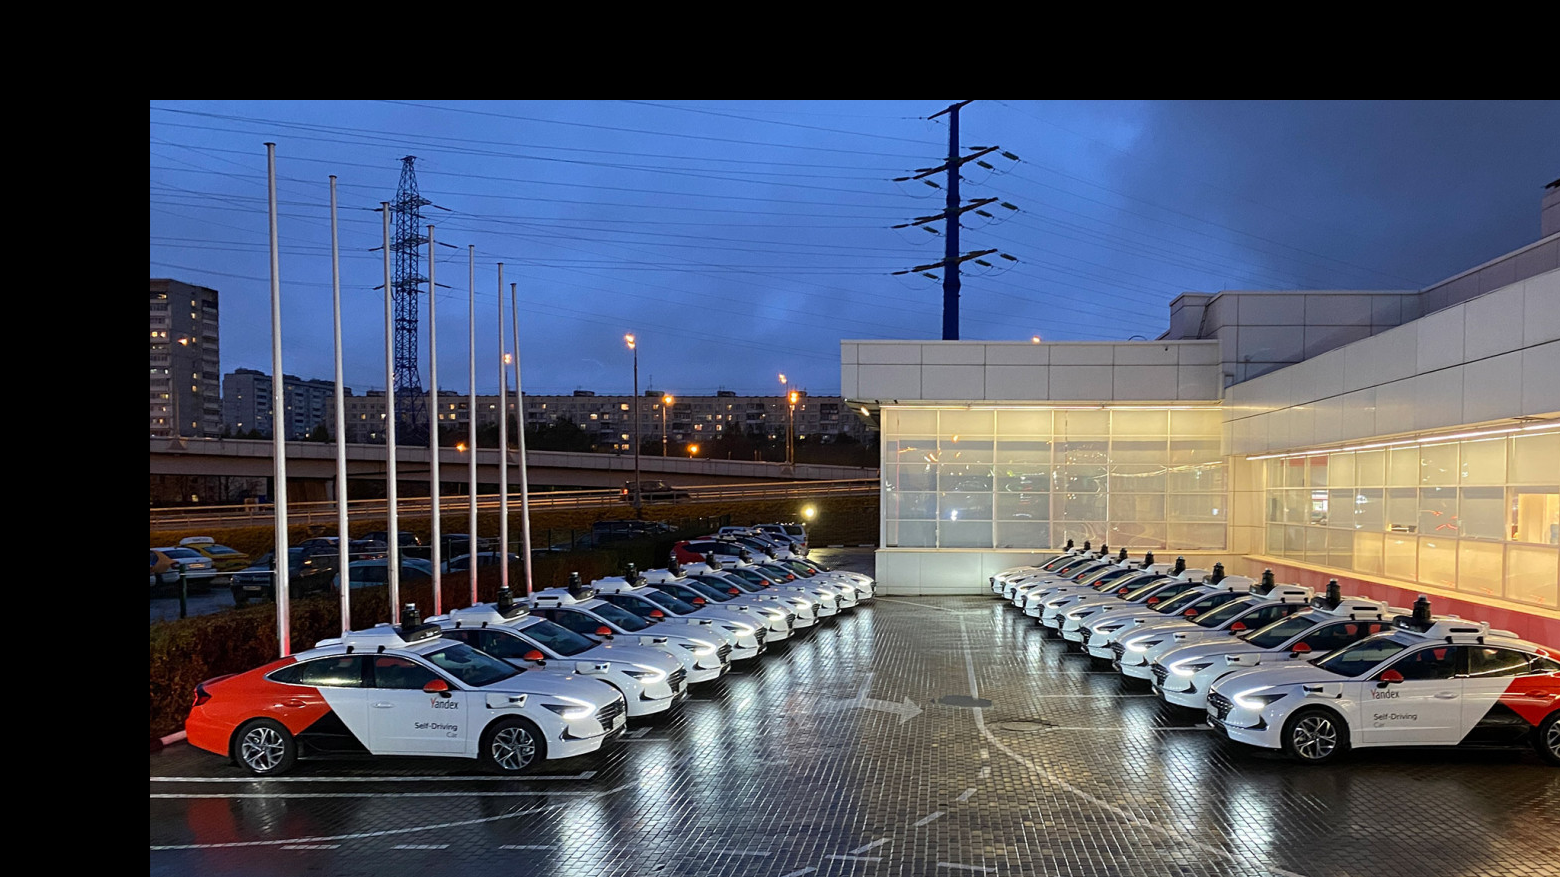
\includegraphics[width=\textwidth]{../outputs/image_shift.png}
    \caption{Сдвиг изображения}
    \label{fig:move_image}
\end{figure}

% \pagebreak
\subsection{Отражение изображения}

Отражение изображения относительно оси OX можно получить с помощью следующей матрицы преобразования:
\begin{equation}
T = \begin{bmatrix}
    1 & 0 & 0 \\
    0 & -1 & h - 1 \\
    0 & 0 & 1
\end{bmatrix}
\end{equation}
где $h$ -- высота изображения.

Отражение изображения относительно оси OY можно получить с помощью следующей матрицы преобразования:
\begin{equation}
T = \begin{bmatrix}
    -1 & 0 & w - 1 \\
    0 & 1 & 0 \\
    0 & 0 & 1
\end{bmatrix}  
\end{equation}
где $w$ -- ширина изображения.

Использование коэффициентов $h - 1$ и $w - 1$ обусловлено тем, что нам необходимо, чтобы после отражения изображение оставалось в пределах координатной сетки.


Рассмотрим как применить отражение изображения относительно оси OX и OY:

\begin{lstlisting}[style=cpp_white, caption={Исходный код для отражения изображения относительно оси OX}]
    T = (cv::Mat_<double>(2, 3) << 
                1, 0, 0, 
             0, -1, image.rows-1); 

    cv::warpAffine(image, image_reflect, T, cv::Size(image.cols, image.rows));

    cv::imwrite(path + "/lab2/outputs/image_reflect.png", image_reflect);

    cv::imshow("Shift image", image_reflect); 
    cv::waitKey(0); 
\end{lstlisting}

\begin{figure}[ht]
    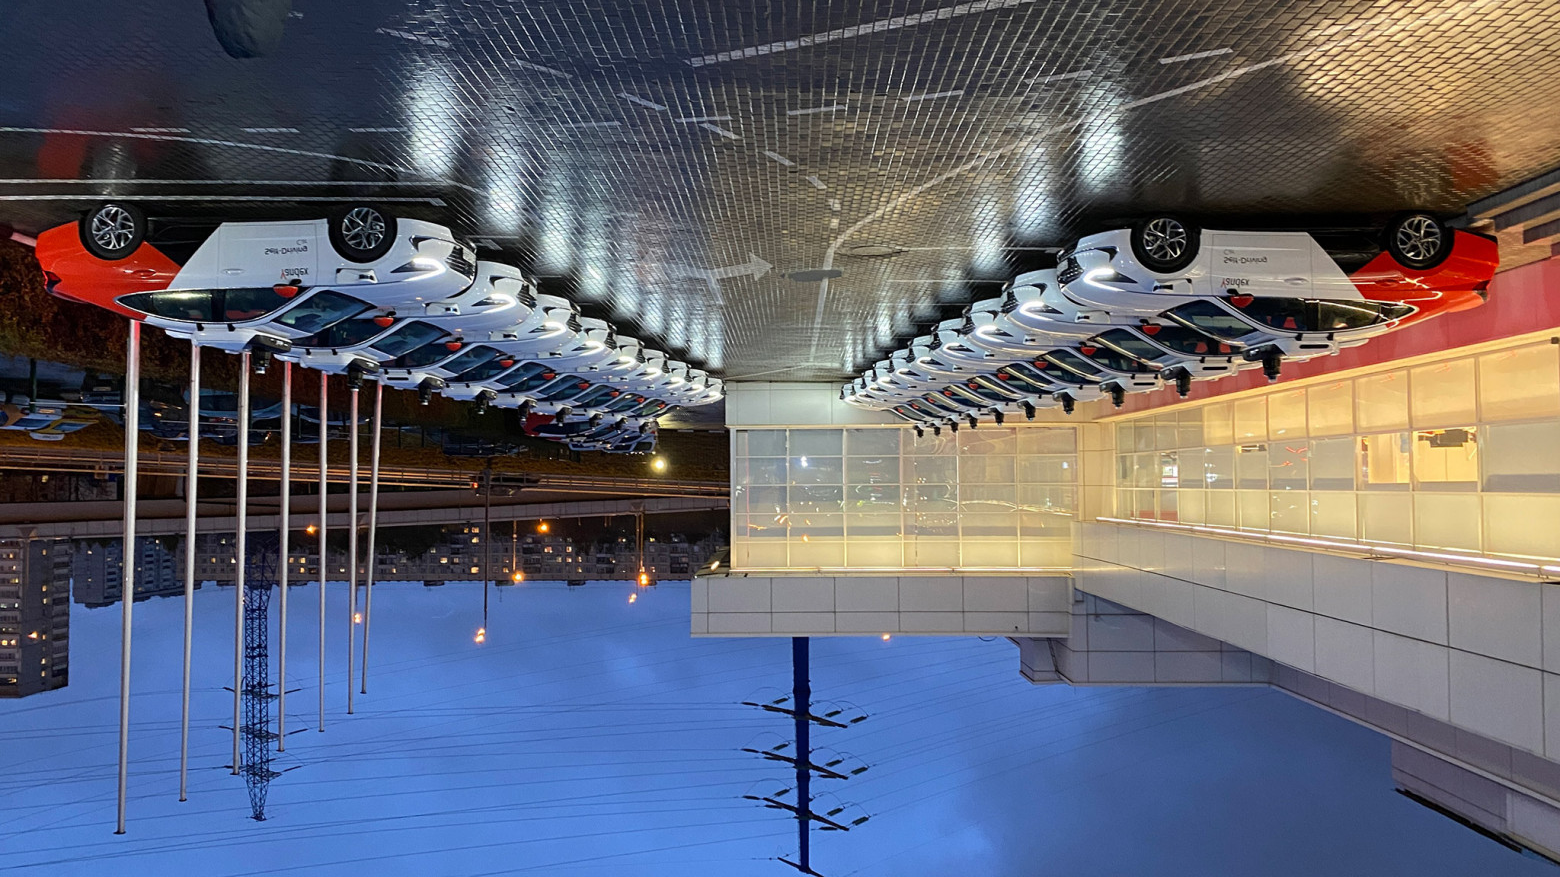
\includegraphics[width=\textwidth]{../outputs/image_reflect.png}
    \caption{Отражение изображения относительно оси OX}
    \label{fig:mirror_image_x}
\end{figure}

% \pagebreak
\begin{lstlisting}[style=cpp_white, caption={Исходный код для отражения изображения относительно оси OY}]
cv::flip(image, image_reflect, 1);

cv::imwrite(path + "/lab2/outputs/image_flip.png", image_reflect);

cv::imshow("Shift image", image_reflect); 
cv::waitKey(0); 
\end{lstlisting}

\begin{figure}[ht]
    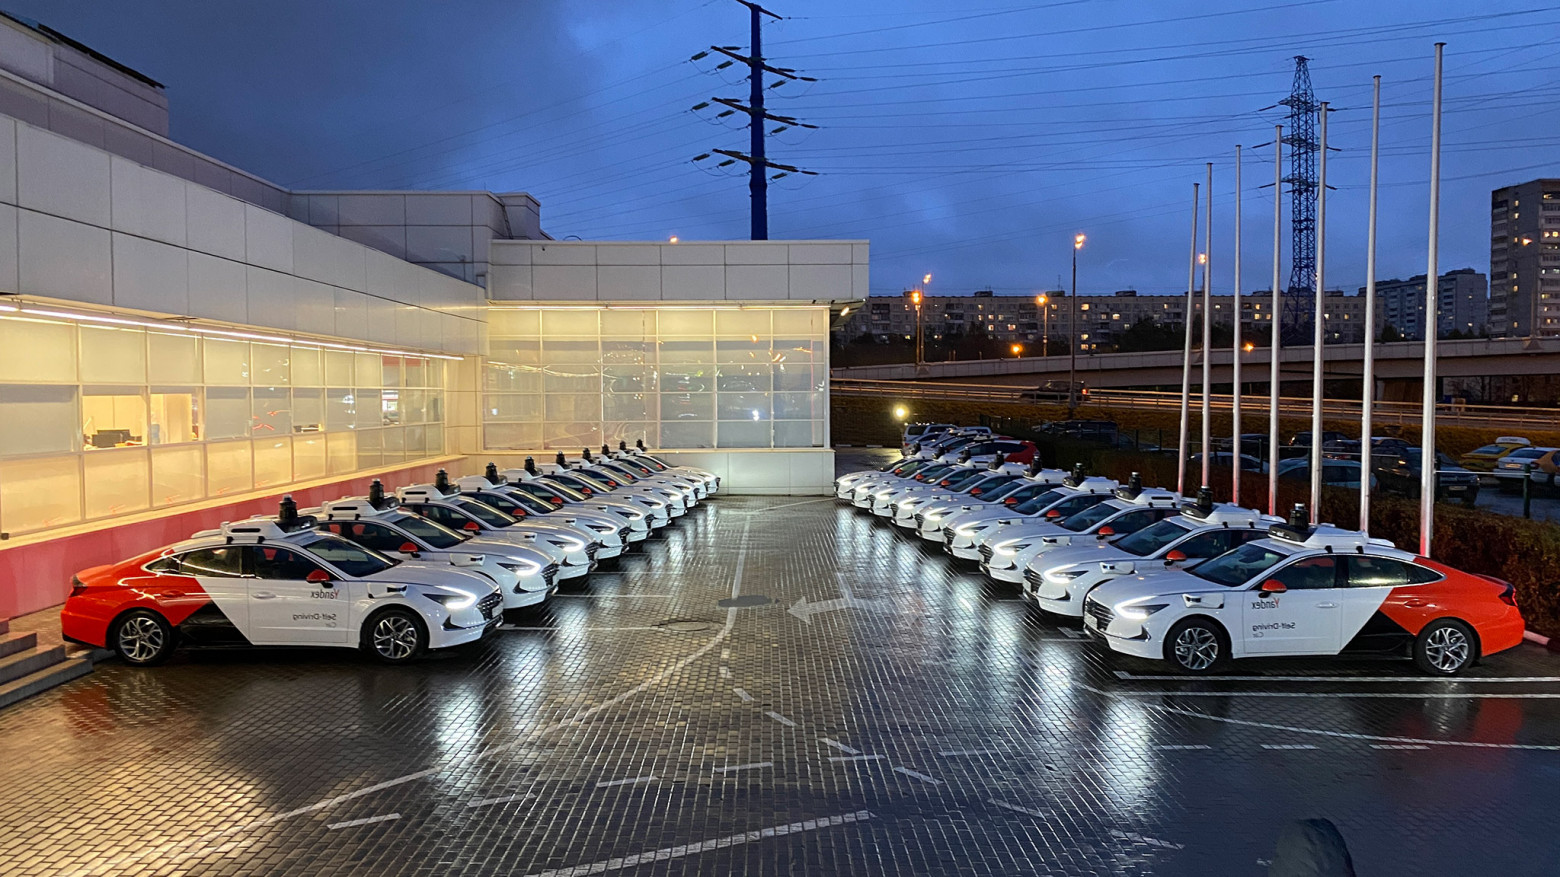
\includegraphics[width=\textwidth]{../outputs/image_flip.png}
    \caption{Отражение изображения относительно оси OY}
    \label{fig:mirror_image_Y}
\end{figure}

% \pagebreak
\subsection{Однородное масштабирование изображения}

Для однородного масштабирования изображения на коэффициент $s$ необходимо использовать следующую матрицу преобразования:
\begin{equation}
T = \begin{bmatrix}
    s & 0 & 0 \\
    0 & s & 0 \\
    0 & 0 & 1
\end{bmatrix}
\end{equation}

Рассмотрим как применить однородное масштабирование изображения с коэффициентом 0.5:
\begin{lstlisting}[style=cpp_white, caption={Исходный код для однородного масштабирования изображения}]
T = (cv::Mat_<double>(2, 3) << 
                    0.5, 0, 0, 
                    0, 0.5, 0); 

cv::warpAffine(image, image_scale, T, cv::Size(int(0.5 * image.cols), int(0.5 * image.rows))); 

cv::imwrite(path + "/lab2/outputs/image_scale.png", image_scale);

cv::imshow("Shift image", image_scale); 
cv::waitKey(0);
\end{lstlisting}

\begin{figure}[ht]
    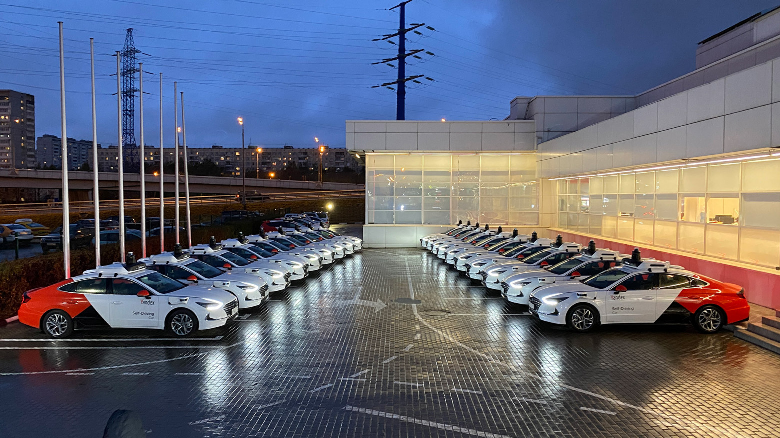
\includegraphics[width=\textwidth]{../outputs/image_scale.png}
    \caption{Однородное масштабирование изображения}
    \label{fig:uniform_scale_image}
\end{figure}

Кроме того, можно использовать функцию \texttt{cv::resize} из библиотеки OpenCV для однородного масштабирования изображения:
\begin{lstlisting}[style=cpp_white, caption={Исходный код для однородного масштабирования изображения с использованием библиотеки OpenCV}]
cv::resize(image, image_resize, cv::Size(int(0.5 * image.cols), int(0.5 * image.rows)));

cv::imwrite(path + "/lab2/outputs/image_resize.png", image_resize);

cv::imshow("Shift image", image_resize); 
cv::waitKey(0); 
\end{lstlisting}

\begin{figure}[ht]
    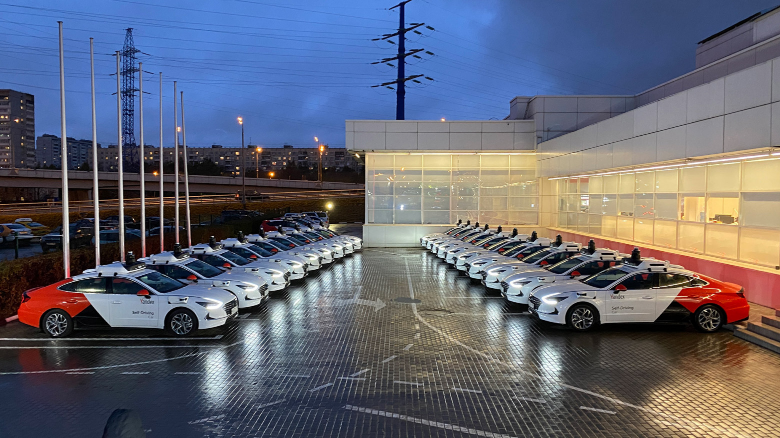
\includegraphics[width=\textwidth]{../outputs/image_resize.png}
    \caption{Однородное масштабирование изображения с использованием библиотеки OpenCV}
    \label{fig:uniform_scale_image_cv}
\end{figure}

% \pagebreak
\subsection{Поворот изображения}

Для поворота изображения на угол $\theta$ необходимо использовать следующую матрицу преобразования:

\begin{equation}
T = \begin{bmatrix}
    \cos(\theta) & -\sin(\theta) & 0 \\
    \sin(\theta) & \cos(\theta) & 0 \\
    0 & 0 & 1
\end{bmatrix}
\end{equation}

Рассмотрим как применить поворот изображения на 25 градусов:
\begin{lstlisting}[style=cpp_white, caption={Исходный код для поворота изображения}]
double phi = 25 * M_PI / 180;
T = (cv::Mat_<double>(2, 3) << 
    cos(phi), -sin(phi), 0, 
    sin(phi), cos(phi), 0); 

cv::warpAffine(image, image_rotate, T, cv::Size(image.cols, image.rows)); 

cv::imwrite(path + "/lab2/outputs/image_rotate.png", image_rotate);

cv::imshow("Shift image", image_rotate); 
cv::waitKey(0); 
\end{lstlisting}

\begin{figure}[ht]
    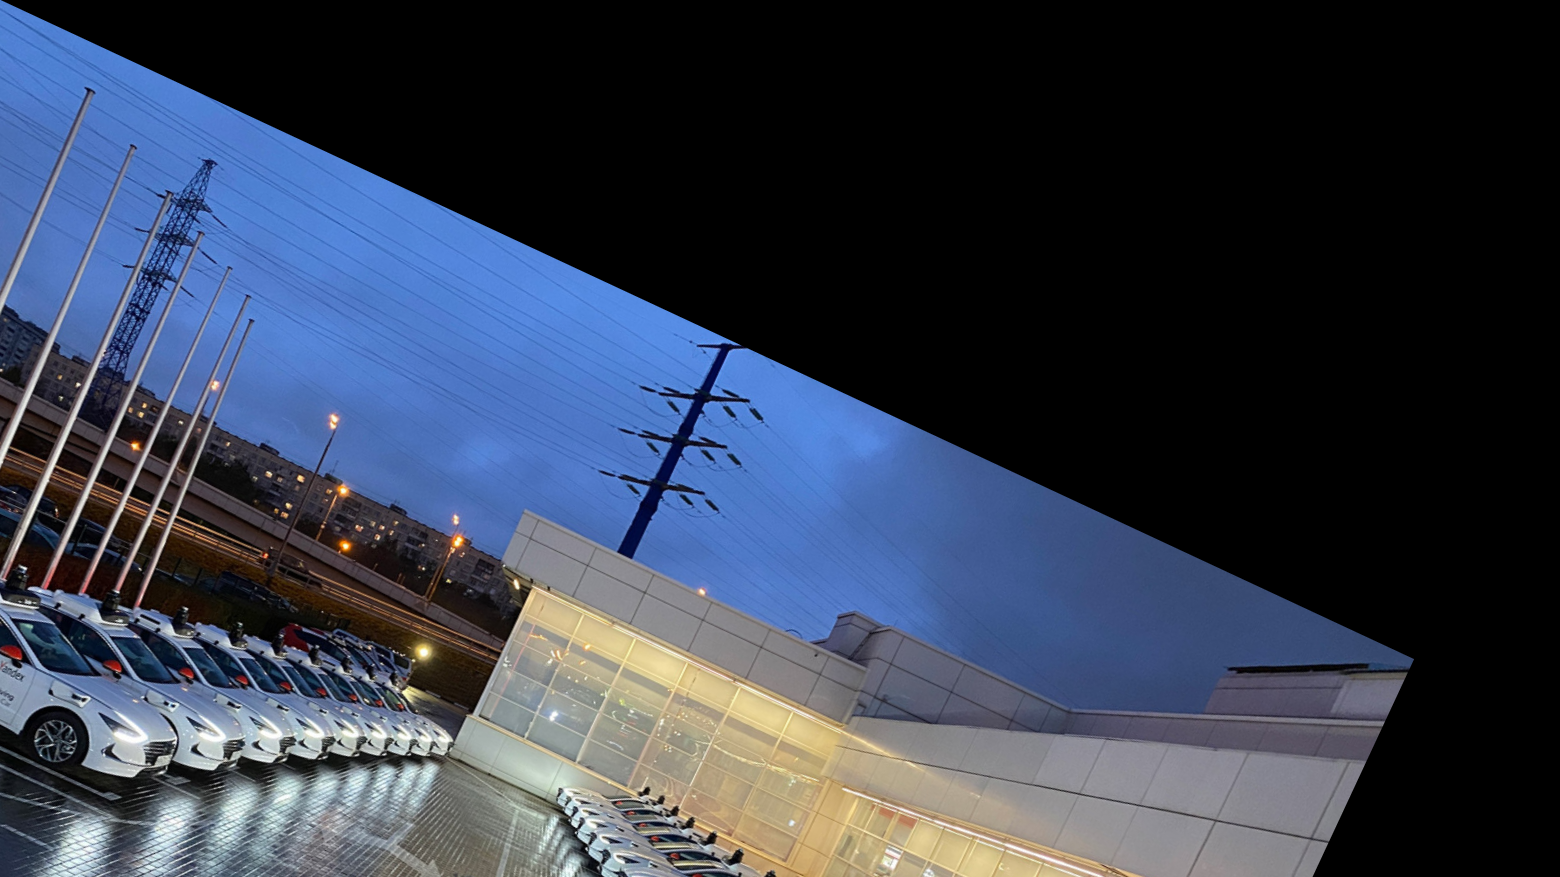
\includegraphics[width=\textwidth]{../outputs/image_rotate.png}
    \caption{Поворот изображения}
    \label{fig:rotate_image}
\end{figure}

Видим, что изображения действительно повернулось на 25 градусов против часовой стрелки относительно начала координат, 
которое находится в левом верхнем углу изображения.

Для того, чтобы осуществить поворот изображения относительно определенной точки, необходимо выполнить следующие шаги:

\begin{enumerate}
    \item Переместить изображение так, чтобы точка, относительно которой будет осуществляться поворот, находилась в начале координат
    \item Повернуть изображение относительно начала координат
    \item Переместить изображение обратно
\end{enumerate}

Матрицы для каждого шага будут следующими:
\begin{equation}
T_1 = \begin{bmatrix}
    1 & 0 & -\frac{w}{2} \\
    0 & 1 & -\frac{h}{2} \\
    0 & 0 & 1
\end{bmatrix}
\end{equation}
\begin{equation}
T_2 = \begin{bmatrix}
    \cos(\theta) & -\sin(\theta) & 0 \\
    \sin(\theta) & \cos(\theta) & 0 \\
    0 & 0 & 1
\end{bmatrix}
\end{equation}
\begin{equation}
T_3 = T_1^{-1} = \begin{bmatrix}
    1 & 0 & \frac{w}{2} \\
    0 & 1 & \frac{h}{2} \\
    0 & 0 & 1
\end{bmatrix}
\end{equation}
Применение этих матриц к изображению позволит осуществить поворот изображения относительно центра:
\begin{equation}
    X' = T_3 \times T_2 \times T_1 \times I
\end{equation}

Рассмотрим как применить поворот изображения на 10 градусов относительно центра:
\begin{lstlisting}[style=cpp_white, caption={Исходный код для поворота изображения с использованием библиотеки OpenCV}]
double phi = 25 * M_PI / 180;

T1 = (cv::Mat_<double>(3, 3) << 
    1, 0, -(image.cols-1) / 2.0, 
    0, 1, -(image.rows-1) / 2.0,
    0, 0, 1); 

T2 = (cv::Mat_<double>(3, 3) << 
    cos(phi), -sin(phi), 0, 
    sin(phi), cos(phi), 0,
    0, 0, 1);  

T3 = (cv::Mat_<double>(3, 3) << 
    1, 0, (image.cols-1) / 2.0, 
    0, 1, (image.rows-1) / 2.0,
    0, 0, 1);   

T = cv::Mat(T3 * T2 * T1, cv::Rect(0, 0, 3, 2));

cv::warpAffine(image, image_rotate_point, T, cv::Size(image.cols, image.rows)); 

cv::imwrite(path + "/lab2/outputs/image_rotate_point.png", image_rotate_point);

cv::imshow("Shift image", image_rotate_point); 
cv::waitKey(0); 
\end{lstlisting}

\begin{figure}[ht]
    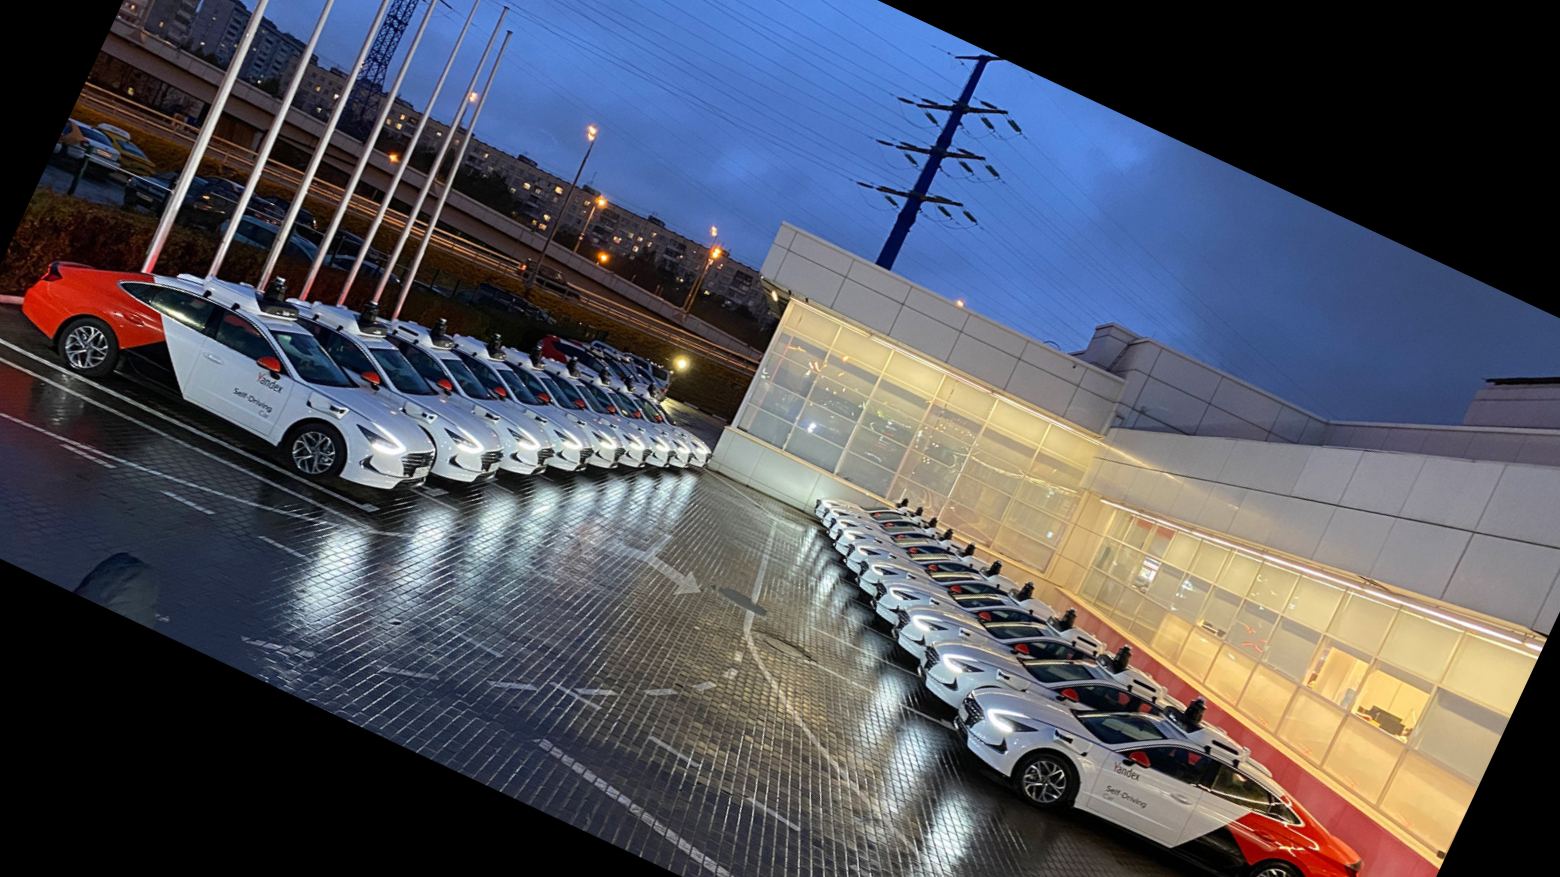
\includegraphics[width=\textwidth]{../outputs/image_rotate_point.png}
    \caption{Поворот изображения относительно центра}
    \label{fig:rotate_image_center}
\end{figure}

Кроме того, можно использовать функцию \texttt{cv2.getRotationMatrix2D} из библиотеки OpenCV для поворота изображения относительно центра:
\begin{lstlisting}[style=cpp_white, caption={Исходный код для поворота изображения относительно центра с использованием библиотеки OpenCV}]
double phi = 25;
T = cv::getRotationMatrix2D(cv::Point2d(((image.cols-1) / 2.0), (image.rows-1) / 2.0), -phi, 1);
cv::warpAffine(image, image_rotate_point_func, T, cv::Size(image.cols, image.rows)); 

cv::imwrite(path + "/lab2/outputs/image_rotate_point_func.png", image_rotate_point_func);

cv::imshow("Shift image", image_rotate_point_func); 
cv::waitKey(0); 
\end{lstlisting}

\begin{figure}[ht]
    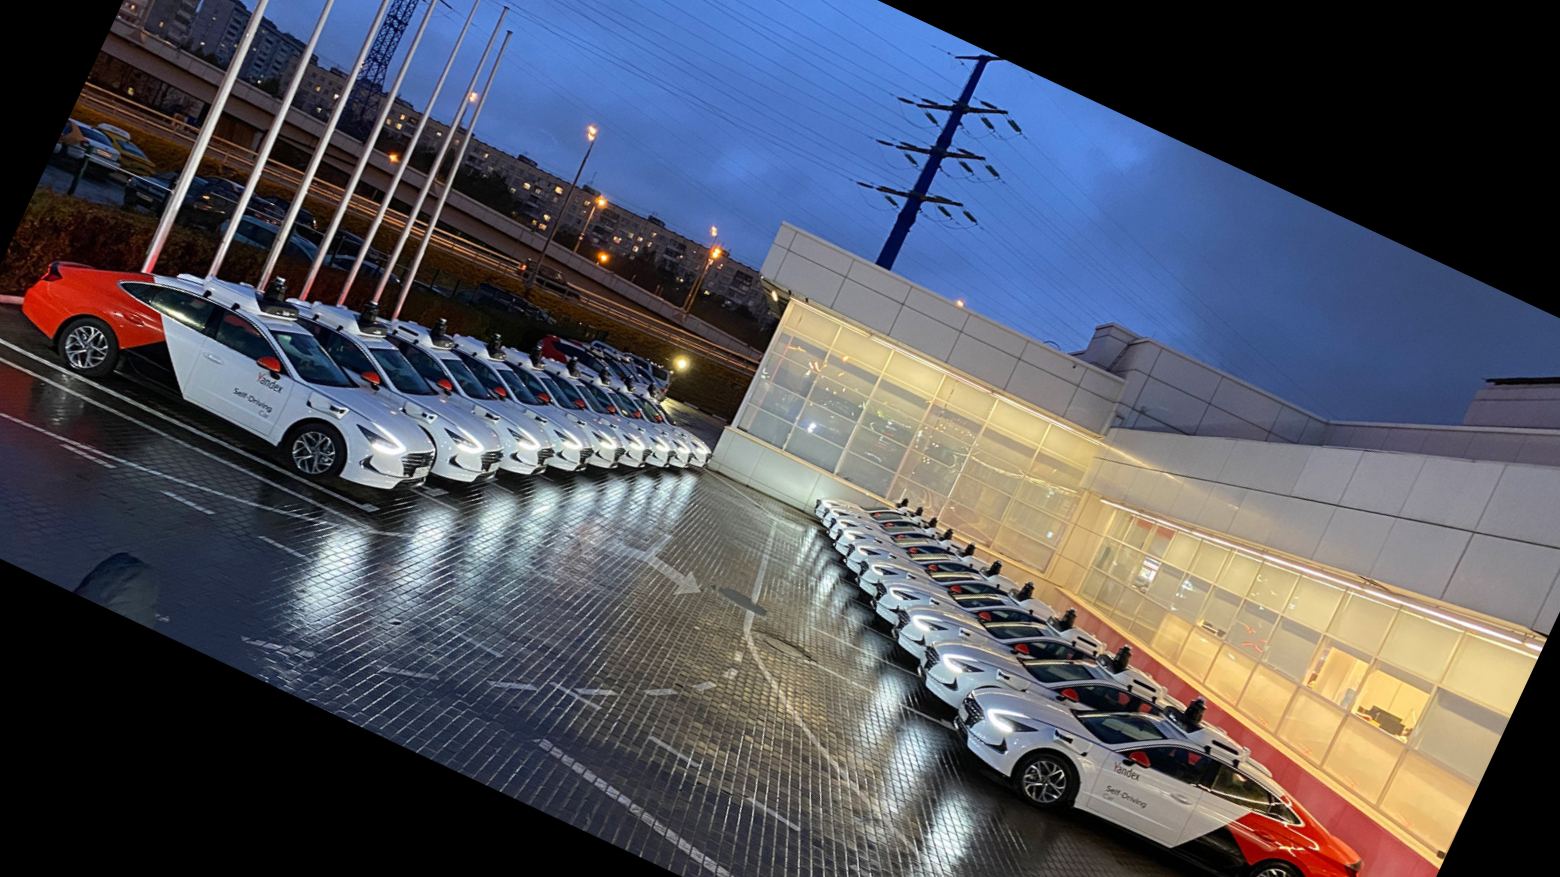
\includegraphics[width=\textwidth]{../outputs/image_rotate_point_func.png}
    \caption{Поворот изображения с использованием библиотеки OpenCV}
    \label{fig:rotate_image_cv}
\end{figure}

% \pagebreak
\subsection{Аффинное отображение} 

Аффинное преобразование -- это преобразование, которое сохраняет параллельность прямых, соотношение длин отрезков, лежащих на одной прямой, и углы между пересекающимися прямыми.
Аффинные преобразования являются подмножеством проективных преобразований. 

Для задания аффинного преобразования можно использовать три пары соответствующих точек на исходном и преобразованном изображениях.

Программная реализация аффинного преобразования:
\begin{lstlisting}[style=cpp_white, caption={Исходный код для скоса изображения}]
std::vector<cv::Point2f> pts_src = {{50, 300}, 
                                    {150, 200}, 
                                    {50, 50}};
std::vector<cv::Point2f> pts_dst = {{50, 310}, 
                                    {160, 200}, 
                                    {50, 60}};

T = cv::getAffineTransform(pts_src, pts_dst);

cv::warpAffine(image, image_Affine, T, cv::Size(image.cols, image.rows)); 

cv::imwrite(path + "/lab2/outputs/image_Affine.png", image_Affine);

cv::imshow("Shift image", image_Affine); 
cv::waitKey(0); 
\end{lstlisting}

\begin{figure}[ht]
    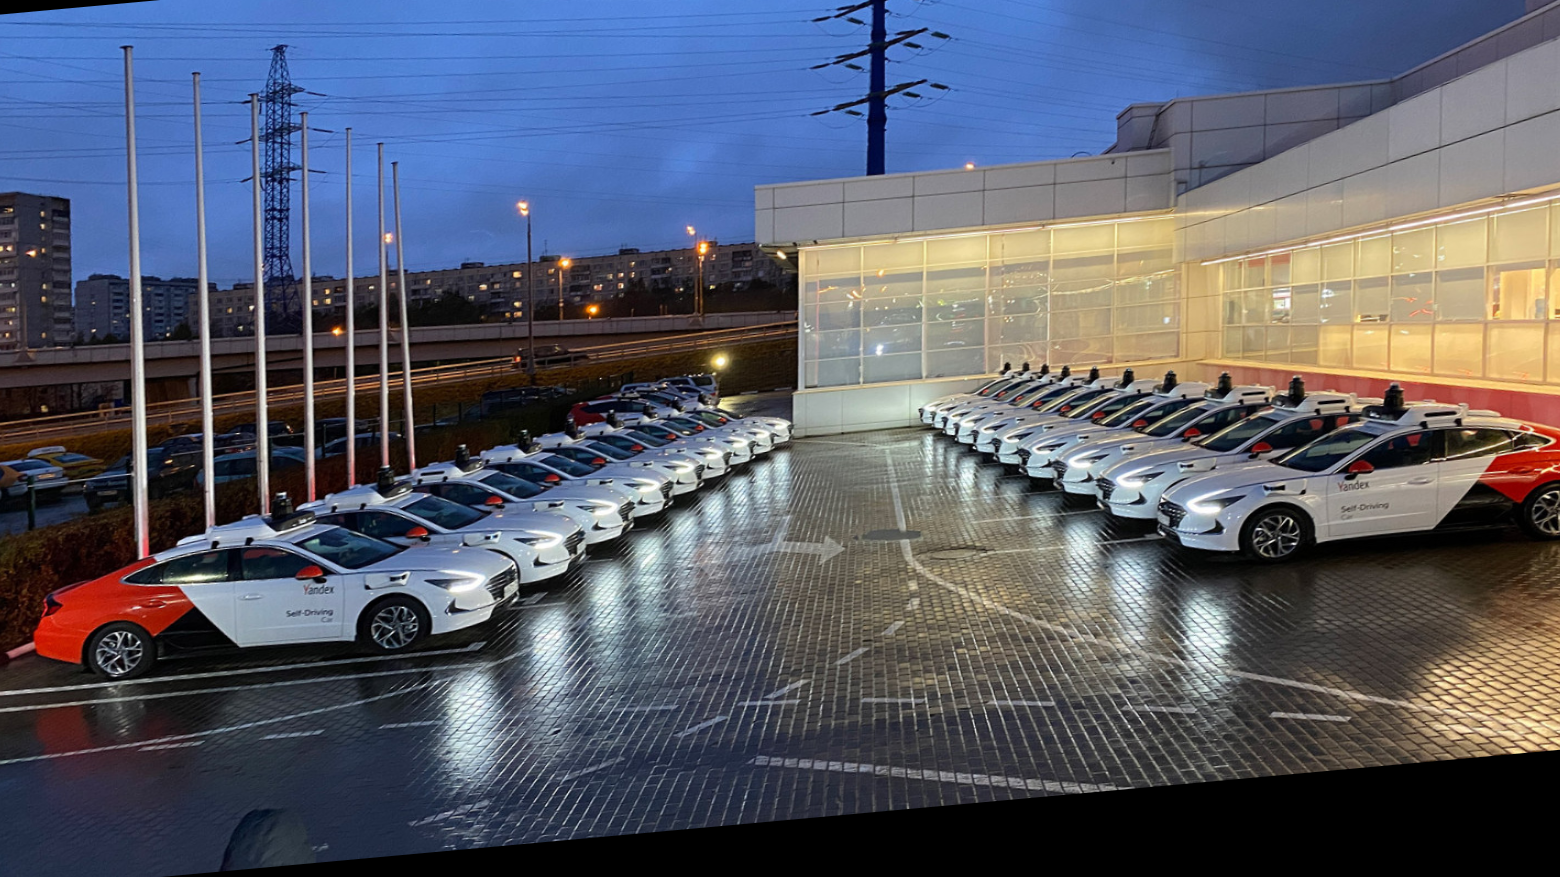
\includegraphics[width=\textwidth]{../outputs/image_Affine.png}
    \caption{Афмнное отображение}
    \label{fig:Affine_image}
\end{figure}

% \pagebreak
\subsection{Скос изображения}

Для того, чтобы осуществить скос изображения, необходимо использовать следующую матрицу преобразования:
\begin{equation}
T_1 = \begin{bmatrix}
    1 & \alpha & 0 \\
    0 & 1 & 0 \\
    0 & 0 & 1
\end{bmatrix} \text{или } 
T_2 = \begin{bmatrix}
    1 & 0 & 0 \\
    \beta & 1 & 0 \\
    0 & 0 & 1
\end{bmatrix}
\end{equation}

Рассмотрим как применить скос изображения:
\begin{lstlisting}[style=cpp_white, caption={Исходный код для скоса изображения}]
double s = 0.2;
T = (cv::Mat_<double>(2, 3) << 
                      1, s, 0, 
                      0, 1, 0); 

cv::warpAffine(image, image_bevel, T, cv::Size(image.cols, image.rows)); 

cv::imwrite(path + "/lab2/outputs/image_bevel.png", image_bevel);

cv::imshow("Shift image", image_bevel); 
cv::waitKey(0);  
\end{lstlisting}

\begin{figure}[ht]
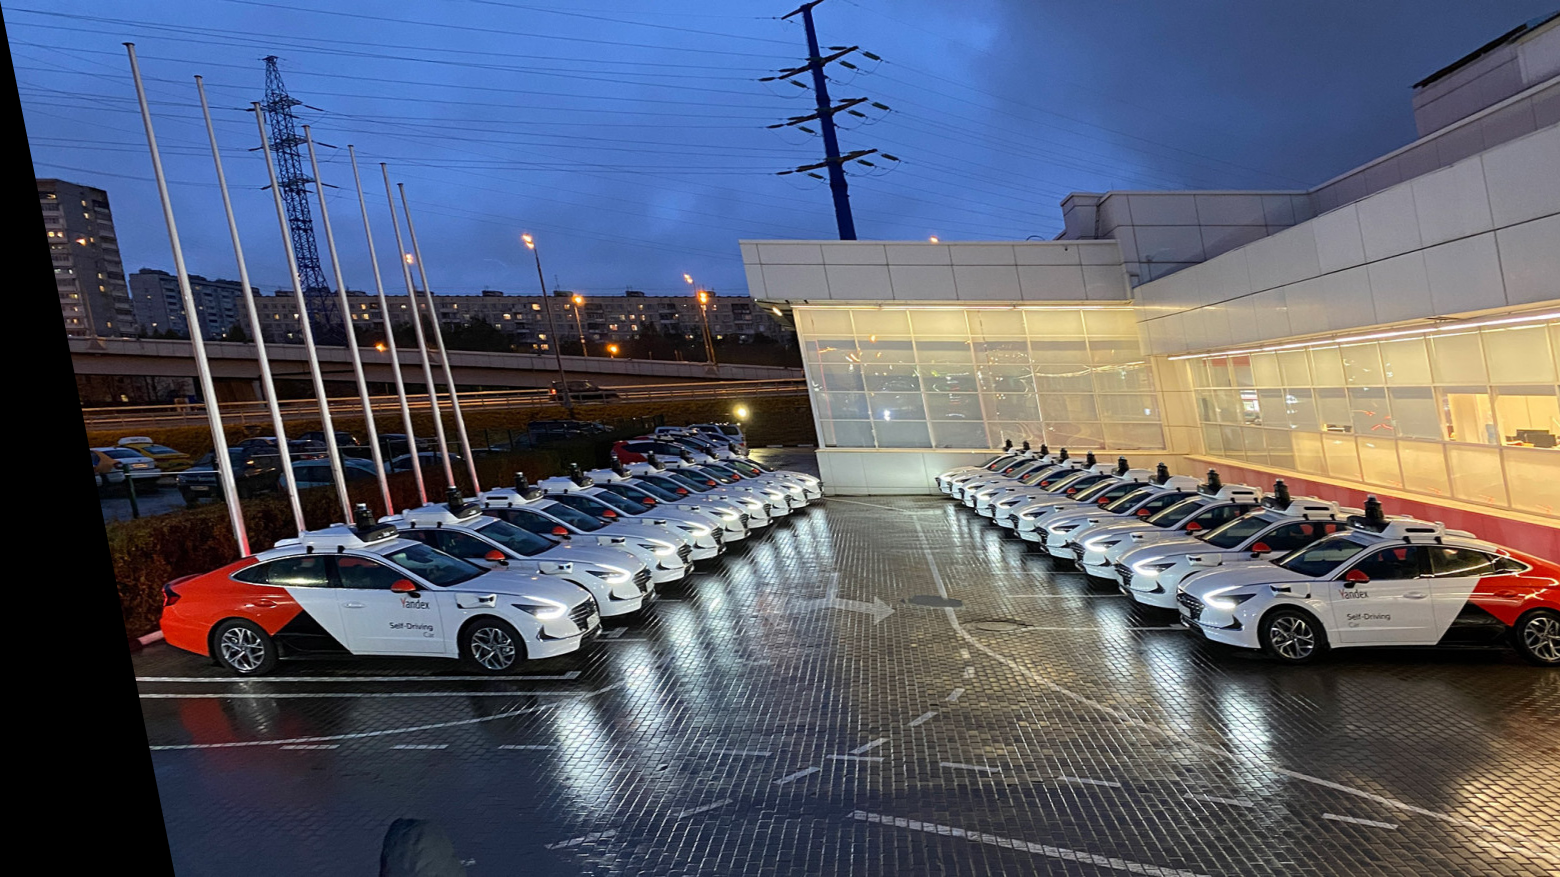
\includegraphics[width=\textwidth]{../outputs/image_bevel.png}
\caption{Скос изображения}
\label{fig:sheared_image}
\end{figure}

\pagebreak
\subsection{Кусочно-линейное преобразование}

Кусочно-линейное преобразование -- это преобразование, при котором изображение разбивает на части, и каждая часть преобразуется отдельно.
Например, можно рассмотреть преобразование, которое левую часть оставляет без изменений, а правую часть растягивает в 4 раза.
\begin{lstlisting}[style=cpp_white, caption={Исходный код для кусочно-линейного преобразования}]
double stretch = 2;
T = (cv::Mat_<double>(2, 3) << 
                stretch, 0, 0, 
                0, 1, 0); 

image_clone = image.clone();
image_piece_r = image_clone(cv::Rect(image.cols / 2, 0, image.cols / 2, image.rows));

cv::warpAffine(image_piece_r, image_piece_r, T, cv::Size(image_piece_r.cols, image.rows)); 

cv::imwrite(path + "/lab2/outputs/image_piece_r.png", image_clone);

cv::imshow("Shift image", image_clone); 
cv::waitKey(0); 
\end{lstlisting}

\begin{figure}[ht]
    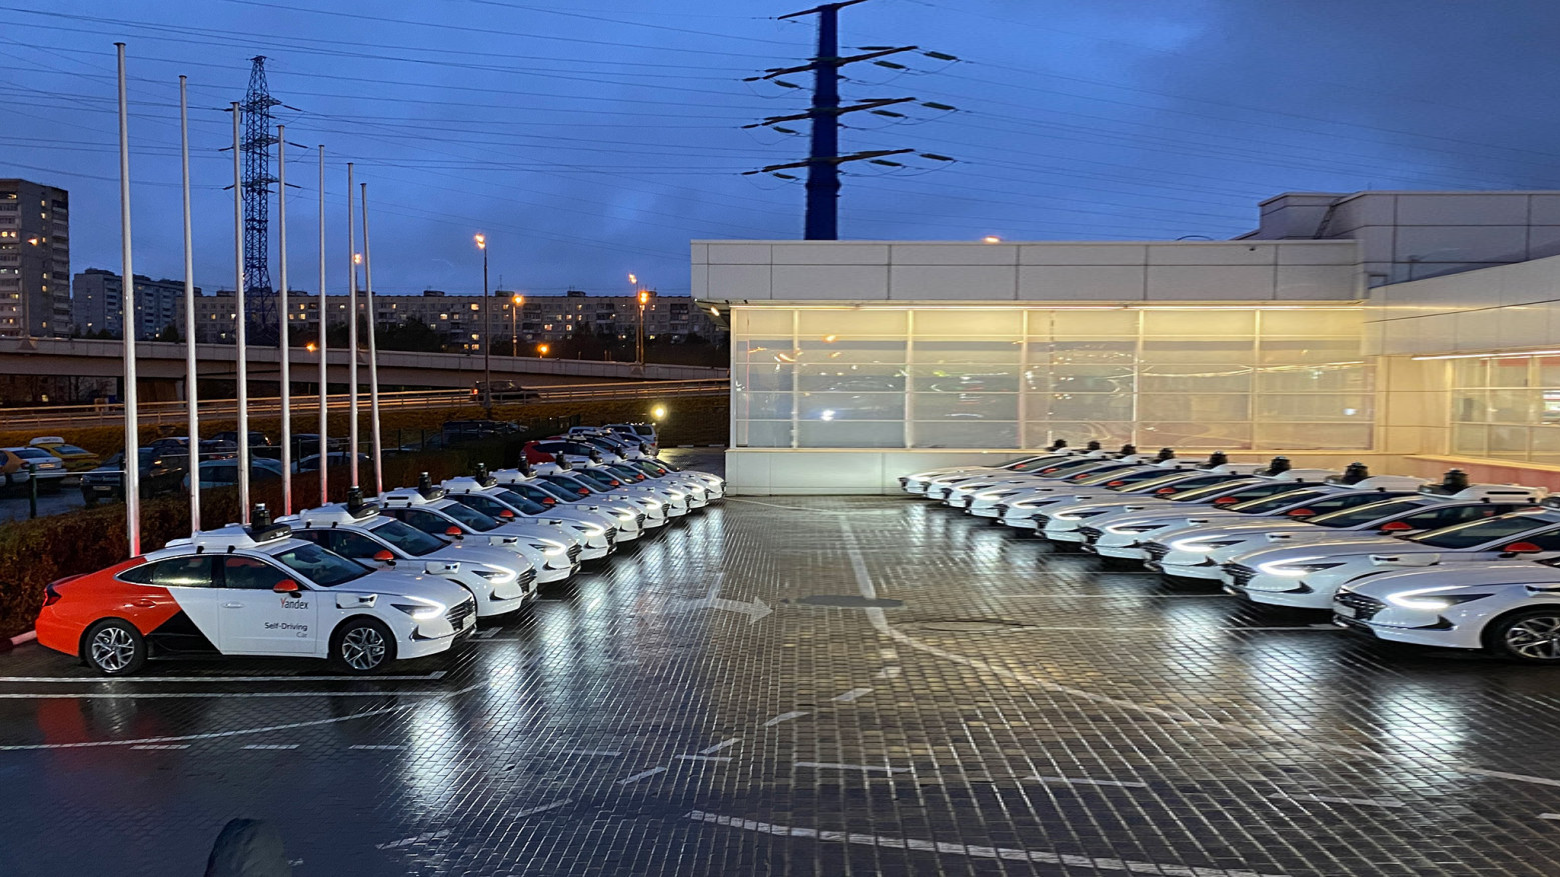
\includegraphics[width=\textwidth]{../outputs/image_piece_r.png}
    \caption{Кусочно-линейное преобразование}
    \label{fig:piecewise_linear_image}
\end{figure}

% \pagebreak
\section{Нелинейные преобразования}

В реальности необходимо применять не только линейные преобразования, но и нелинейные.
Например, для коррекции дисторсии, которая вызывается несовершенством оптики, необходимо использовать нелинейные преобразования.

\subsection{Проекционное отображение}
Проекционное отображение -- это отображение, которое оставляет прямые линии прямыми, но геометрия изображения может быть искажена, так как 
данное отображение не сохраняет углы между прямыми.

Матрица для проекционного отображения в общем виде выглядит следующим образом:

\begin{equation}
T = \begin{bmatrix}
    A & B & E \\
    C & D & F \\
    G & H & K \\
\end{bmatrix}
\end{equation}
где $A, B, C, D$ -- коэффициенты, которые определяют проекционное отображение, $E, F$~--~коэффициенты сдвига, $G, H$~--~коэффициенты, которые определяют проекционный масштаб, $K$~--~коэффициент масштабирования.

Рассмотрим как применить проективное отображение:
\begin{lstlisting}[style=cpp_white, caption={Исходный код для проективного отображения}]
T = (cv::Mat_<double>(3, 3) << 
            0.7, 0.3, 0.00045, 
            0.2, 0.5, 0.0005,
            0, 0, 1); 

cv::warpPerspective(image, image_projective, T, cv::Size(image.cols, image.rows)); 

cv::imwrite(path + "/lab2/outputs/image_projective.png", image_projective);

cv::imshow("Shift image", image_projective); 
cv::waitKey(0); 
\end{lstlisting}

\begin{figure}[ht]
    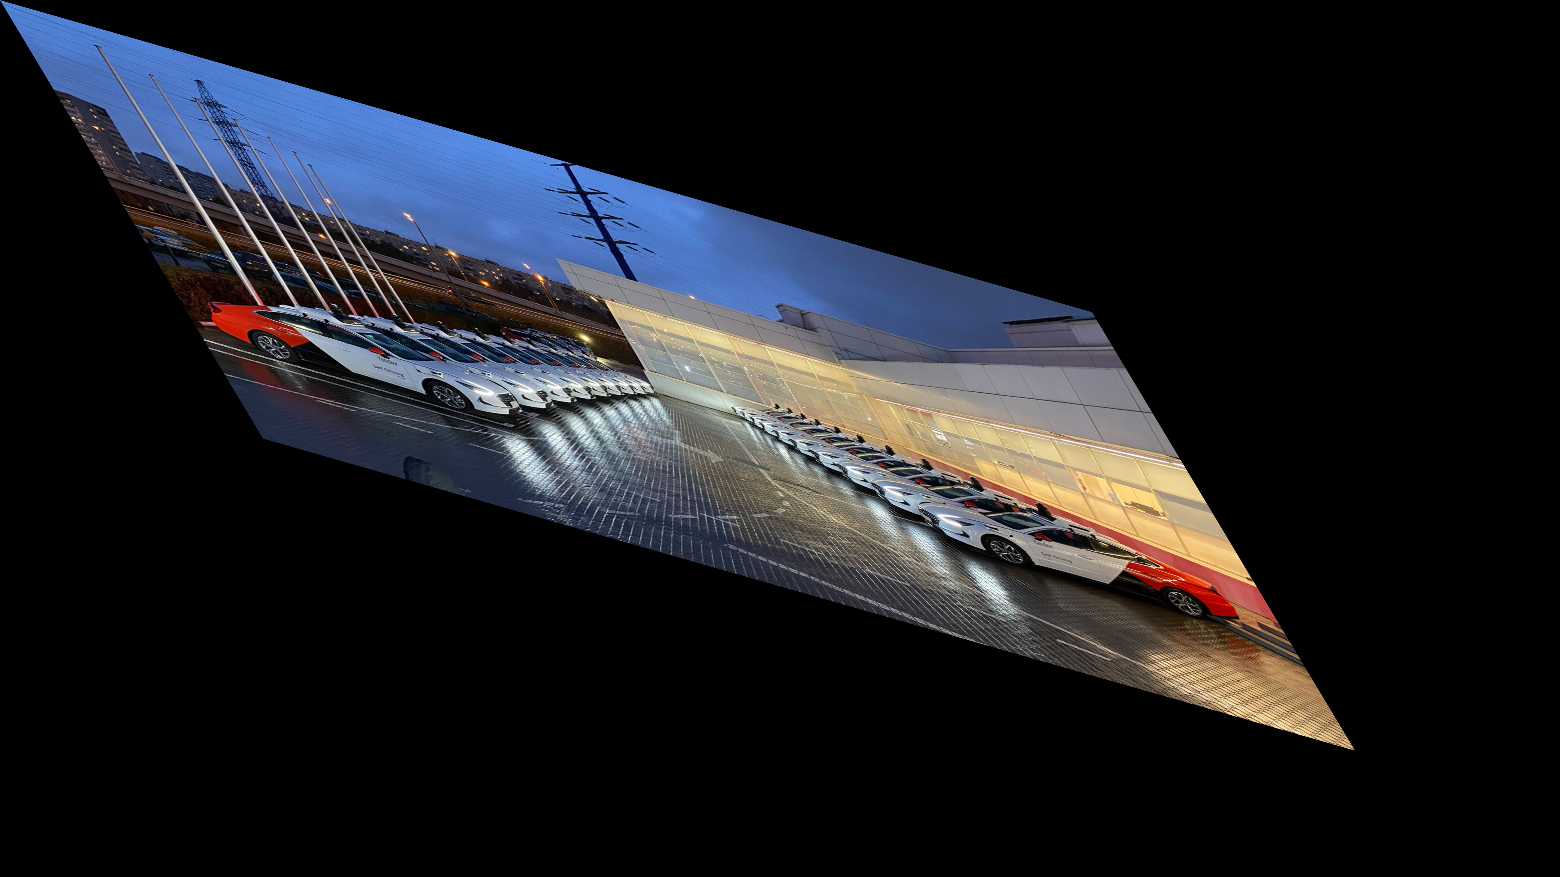
\includegraphics[width=\textwidth]{../outputs/image_projective.png}
    \caption{Проективное отображение}
    \label{fig:projective_image}
\end{figure}

% \pagebreak
\subsection{Полиномиальное преобразование}

Полиномиальное преобразование -- это отображение исходного изображения на преобразованное с использованием полиномиальной функции.

Полиномиальное преобразование второго порядка выглядит следующим образом:
\begin{equation}
\begin{cases}
    x' = a_0 + a_1x + a_2y + a_3x^2 + a_4xy + a_5y^2\\
    y' = b_0 + b_1x + b_2y + b_3x^2 + b_4xy + b_5y^2
\end{cases}
\end{equation}


\begin{lstlisting}[style=cpp_white, caption={Исходный код для полиномиального преобразования}]
const double coeff[2][6] = {{0, 1, 0, 0.00001, 0.0001, 0},
                                        {0, 0, 1, 0, 0.0002, 0}};

if(image.depth() == CV_8U)
    image.convertTo(image_polynomial, CV_32F, 1.0 / 255);
else
    image_polynomial = image;

std::vector<cv::Mat> image_BGR;
cv::split(image_polynomial, image_BGR);
cv::Mat i_pol;
for(int k = 0; k < image_BGR.size(); k++){

    i_pol = cv::Mat::zeros(image_BGR[k].rows, 
                            image_BGR[k].cols, 
                            image_BGR[k].type());

    for(int x = 0; x < image_BGR[k].cols; ++x){
        for(int y = 0; y < image_BGR[k].rows; ++y){

            int x_new = static_cast<int>(round(coeff[0][0] + 
                x * coeff[0][1] + y * coeff[0][2] + 
                x * x * coeff[0][3] + y * x * coeff[0][4] + 
                y * y * coeff[0][5]));

            int y_new = static_cast<int>(round(coeff[1][0] + 
                x * coeff[1][1] + y * coeff[1][2] + 
                x * x * coeff[1][3] + y * x * coeff[1][4] + 
                y * y * coeff[1][5]));

            if(x_new >= 0 && x_new < image_BGR[k].cols
                && y_new >= 0 && y_new < image_BGR[k].rows)
                i_pol.at<float>(y_new, x_new) = image_BGR[k].at<float>(y, x);
        }
    }
    image_BGR[k] = i_pol;
}
cv::merge(image_BGR, i_pol);

if(image.depth() == CV_8U)
    image_polynomial.convertTo(image_polynomial, CV_8UC3, 255);

cv::imwrite(path + "/lab2/outputs/image_polynomial.png", image_polynomial);
cv::imshow("B", image_polynomial);
cv::waitKey(0); 
\end{lstlisting}

\begin{figure}[ht]
    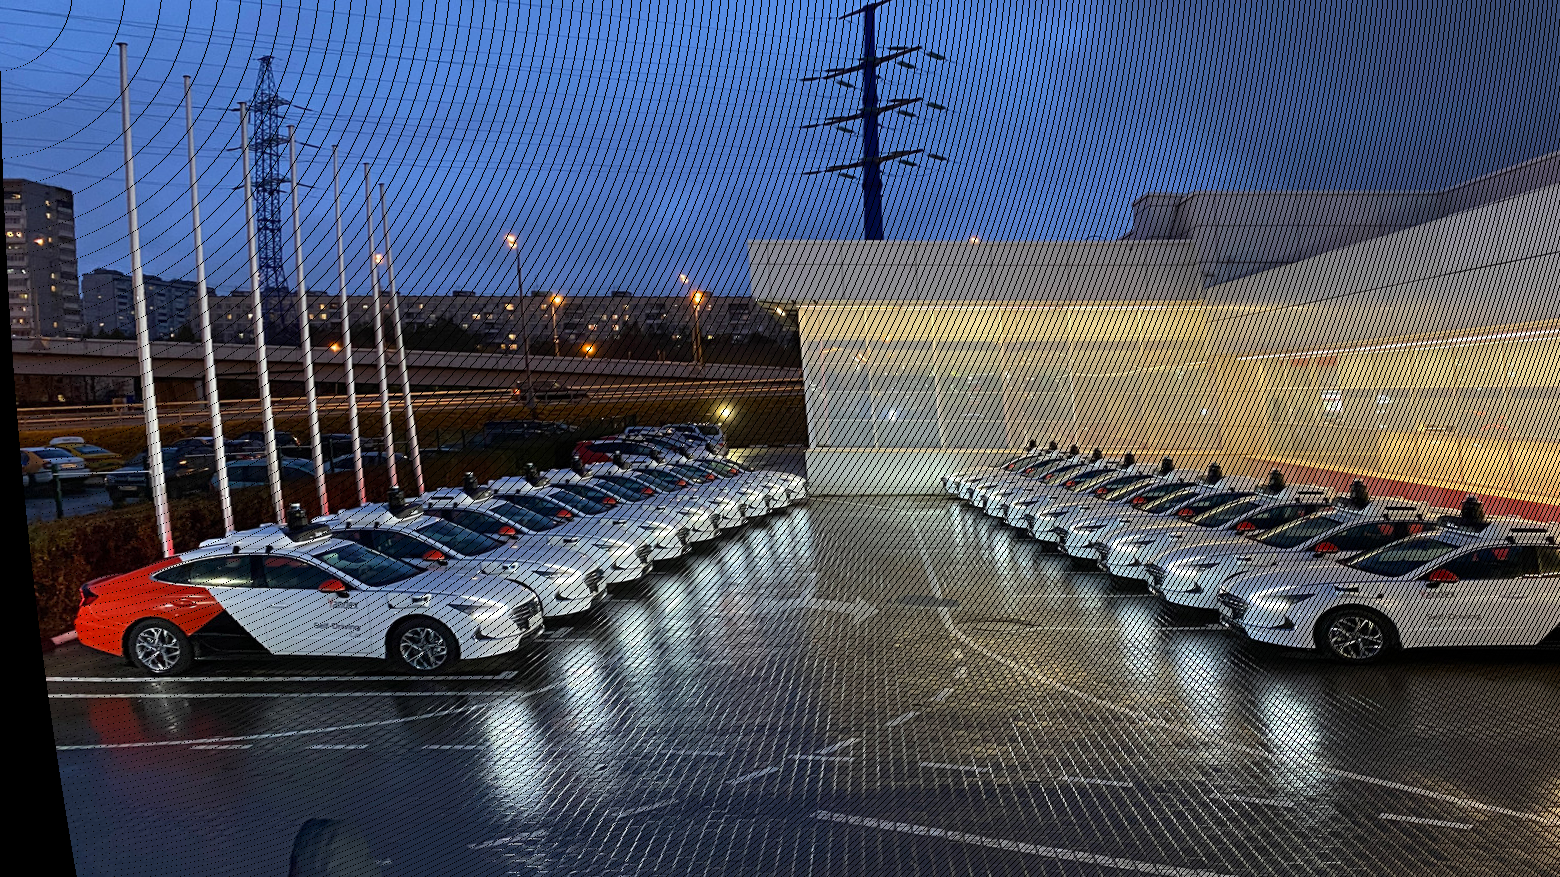
\includegraphics[width=\textwidth]{../outputs/image_polynomial.png}
    \caption{Полиномиальное преобразование}
    \label{fig:polynomial_image}
\end{figure}

Видим, что на изображении появились артефакты, так как не все пиксели были заполнены. Это связано с тем, что при применении полиномиального преобразования
цвета пикселей могут быть не определены для некоторых координат, и в таком случае необходимо использовать интерполяцию.

\pagebreak
\subsection{Синусоидальное искажение}

Еще одним примером нелинейного преобразования может быть искажение изображения по гармоническому закону.

\begin{lstlisting}[style=cpp_white, caption={Исходный код для синусоидального искажения}]
cv::Mat u = cv::Mat::zeros(image.rows, image.cols, CV_32F);
cv::Mat v = cv::Mat::zeros(image.rows, image.cols, CV_32F);

for(int x = 0; x < image.cols; ++x){
    for(int y = 0; y < image.rows; ++y){
        u.at<float>(y, x) = float(x + 20 * sin(2 * M_PI * y / 90));
        v.at<float>(y, x) = float(y);
    }
}
cv::Mat image_sinusoid;
cv::remap(image, image_sinusoid, u, v, cv::INTER_LINEAR);

cv::imwrite(path + "/lab2/outputs/image_sinusoid.png", image_sinusoid);
cv::imshow("B", image_sinusoid);
cv::waitKey(0);
\end{lstlisting}

\begin{figure}[ht]
    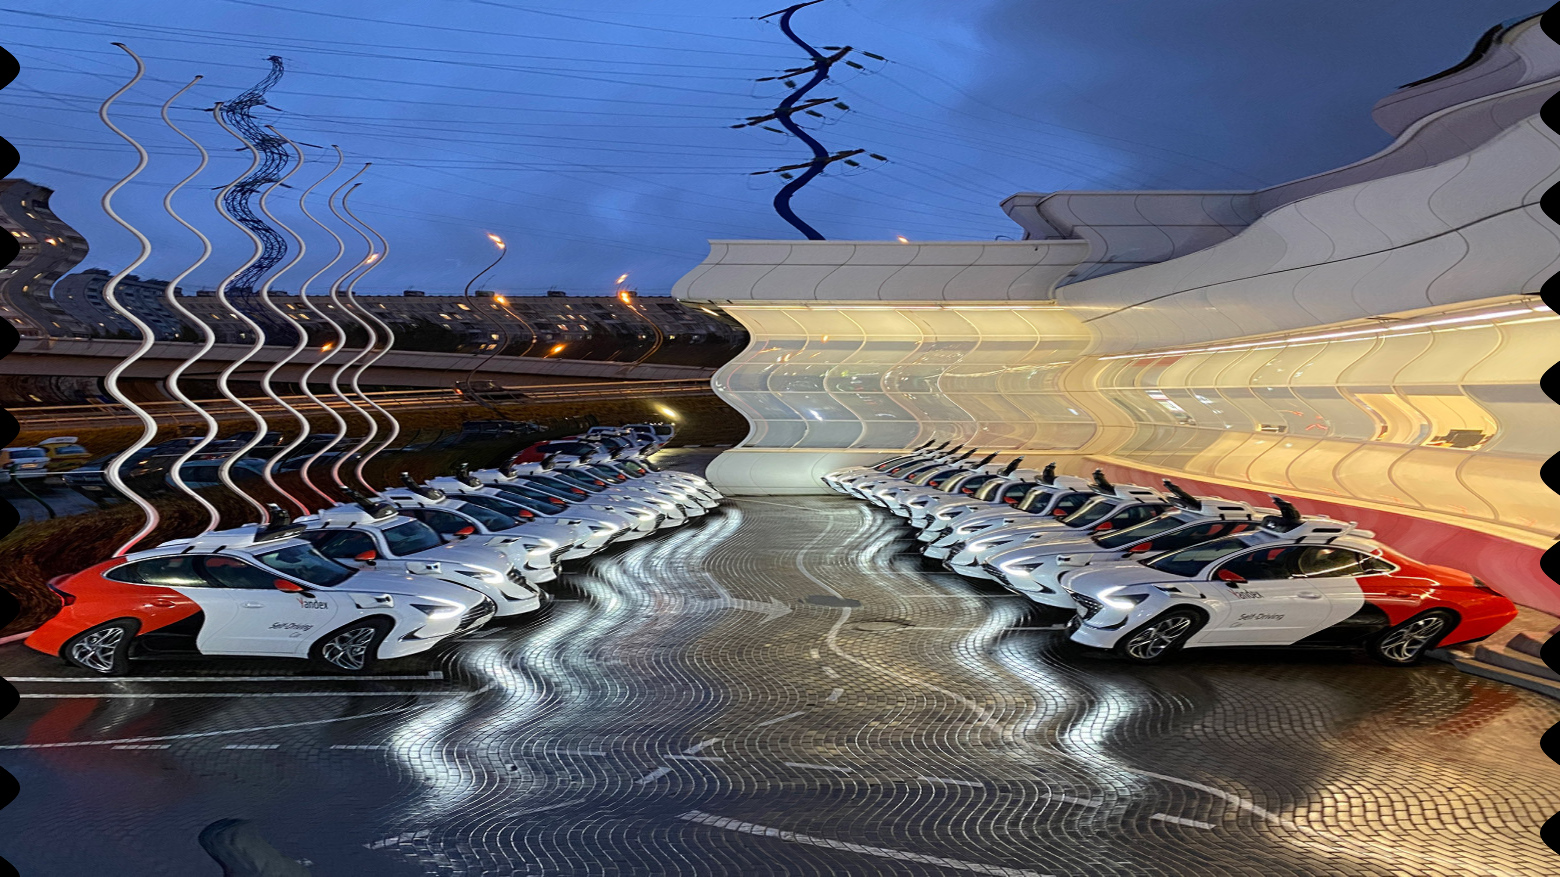
\includegraphics[width=\textwidth]{../outputs/image_sinusoid.png}
    \caption{Синусоидальное искажение}
    \label{fig:sinusoidal_image}
\end{figure}

\pagebreak
\subsection{Коррекция дисторсии}

При формировании изображения оптической системой камеры, на нем может возникнуть дисторсия, которая вызвана несовершенством оптики.
\textbf{Дисторсия} -- это оптическое искажение, которое искривляет прямые линии на изображении.

\begin{lstlisting}[style=cpp_white, caption={Исходный код для коррекции бочкообразной дисторсии}]
cv::Mat x_i, y_i;
std::vector<float> t_x, t_y;

for(int i = 0; i < image.cols; ++i)
    t_x.push_back(float(i));

for(int i = 0; i < image.rows; ++i)
    t_y.push_back(float(i));

cv::repeat(cv::Mat(t_x).reshape(1, 1), image.rows, 1, x_i);
cv::repeat(cv::Mat(t_y).reshape(1, 1).t(), 1, image.cols, y_i);

double x_mid = x_i.cols / 2.0;
double y_mid = x_i.rows / 2.0;

x_i -= x_mid;
x_i /= x_mid;
y_i -= y_mid;
y_i /= y_mid;

cv::Mat r, theta;
cv::cartToPolar(x_i, y_i, r, theta);

double F3 = 0.1, F5 = 0.1;
cv::Mat r3, r5;

pow(r, 3, r3); pow(r, 5, r5);
r += r3 * F3; r += r5 * F5;

cv::Mat u, v;
cv::polarToCart(r, theta, u, v);
u *= x_mid;
u += x_mid;
v *= y_mid;
v *= y_mid;

cv::Mat image_barrel;
cv::remap(image, image_barrel, u, v, cv::INTER_LINEAR);

cv::imwrite(path + "/lab2/outputs/image_barrel.png", image_barrel);
cv::imshow("B", image_barrel);
cv::waitKey(0);
\end{lstlisting}

\begin{figure}[ht]
    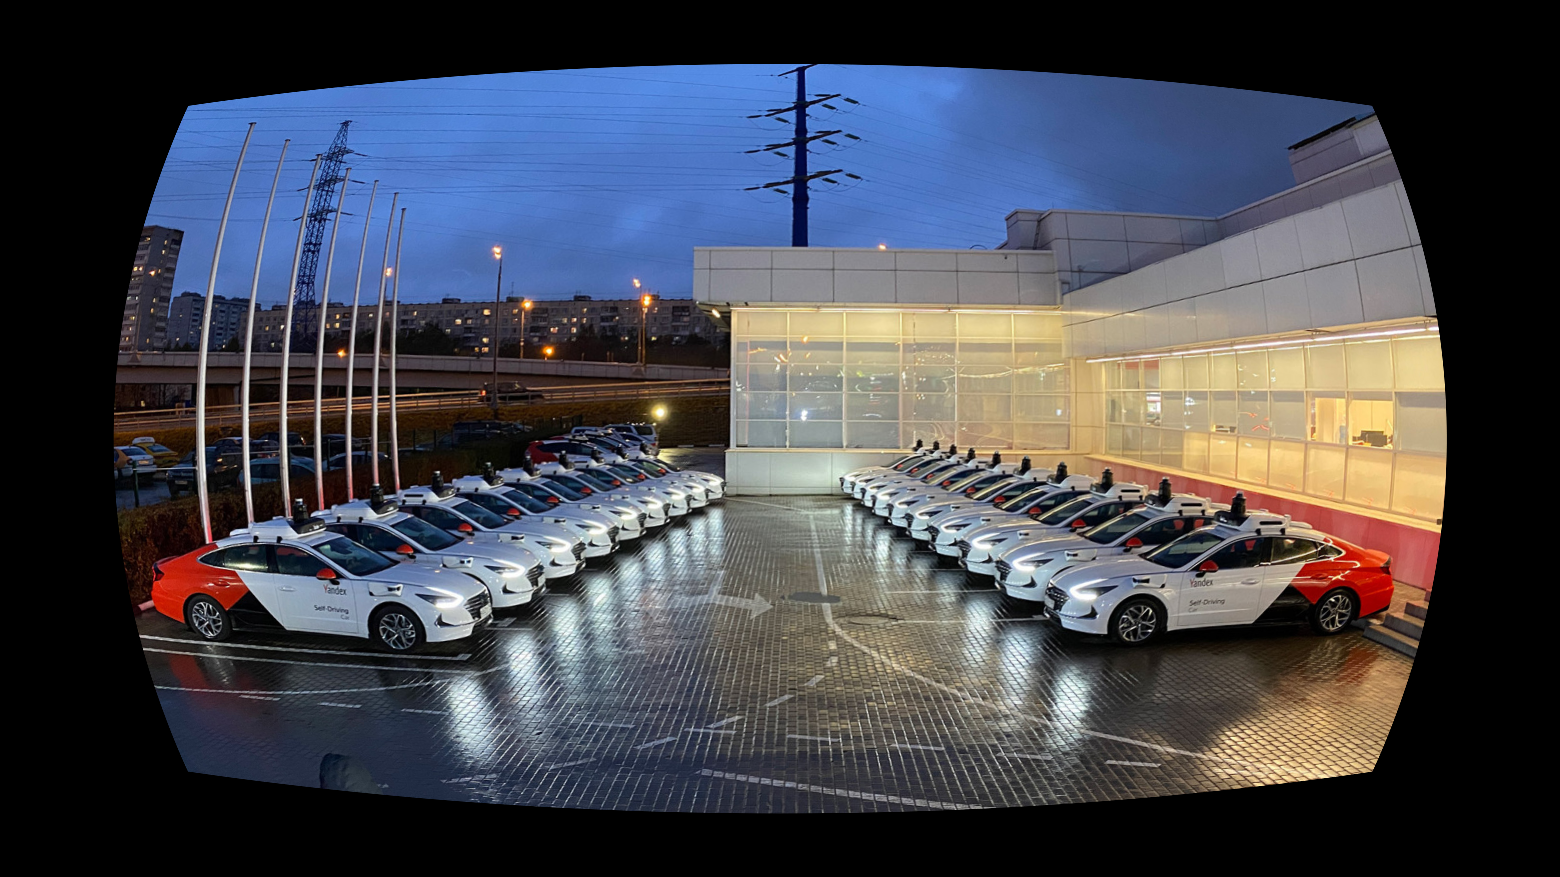
\includegraphics[width=\textwidth]{../outputs/image_barrel.png}
    \caption{Коррекция дисторсии (бочка)}
    \label{fig:distortion_correction_barrel}
\end{figure}

\begin{lstlisting}[style=cpp_white, caption={Исходный код для коррекции подушкообразной дисторсии}]
cv::Mat x_i, y_i;
std::vector<float> t_x, t_y;

for(int i = 0; i < image.cols; ++i)
    t_x.push_back(float(i));

for(int i = 0; i < image.rows; ++i)
    t_y.push_back(float(i));

cv::repeat(cv::Mat(t_x).reshape(1, 1), image.rows, 1, x_i);
cv::repeat(cv::Mat(t_y).reshape(1, 1).t(), 1, image.cols, y_i);

double x_mid = x_i.cols / 2.0;
double y_mid = x_i.rows / 2.0;

x_i -= x_mid;
x_i /= x_mid;
y_i -= y_mid;
y_i /= y_mid;

cv::Mat r, theta;
cv::cartToPolar(x_i, y_i, r, theta);

double F3 = -0.3;
cv::Mat r3, r5;

pow(r, 3, r3); pow(r, 5, r5);
r += r + r3 * F3;

cv::Mat u, v;
cv::polarToCart(r, theta, u, v);
u *= x_mid;
u += x_mid;
v *= y_mid;
v *= y_mid;

cv::Mat image_barrel;
cv::remap(image, image_barrel, u, v, cv::INTER_LINEAR);

cv::imwrite(path + "/lab2/outputs/image_pincushion.png", image_barrel);
cv::imshow("B", image_barrel);
cv::waitKey(0);
\end{lstlisting}

\begin{figure}[ht]
    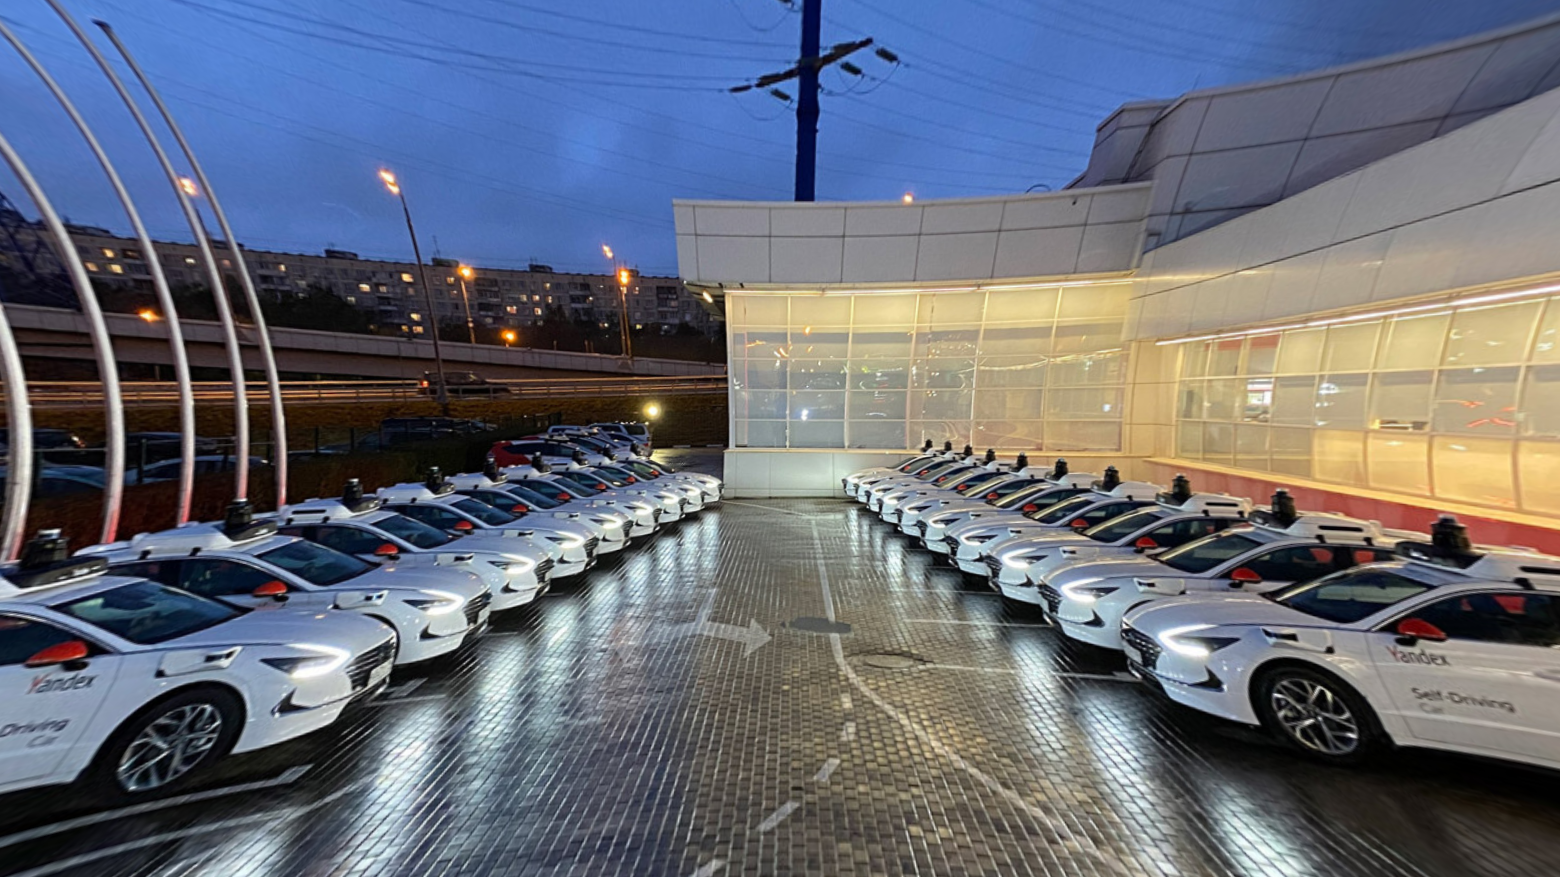
\includegraphics[width=\textwidth]{../outputs/image_pincushion.png}
    \caption{Коррекция дисторсии (подушка)}
    \label{fig:distortion_correction_pincushion}
\end{figure}

\pagebreak
\section{Сшивка изображений}

Сшивка изображений -- это процесс объединения двух или более изображений в одно.
Для того, чтобы осуществить сшивку изображений, необходимо найти общие точки на изображениях, и на основе этих точек осуществить сшивку, 
перейдя от системы координат одного изображения к системе координат другого изображения.

Посмотрим на два изображения, которые необходимо сшить:

\begin{figure}[ht]
    \centering
    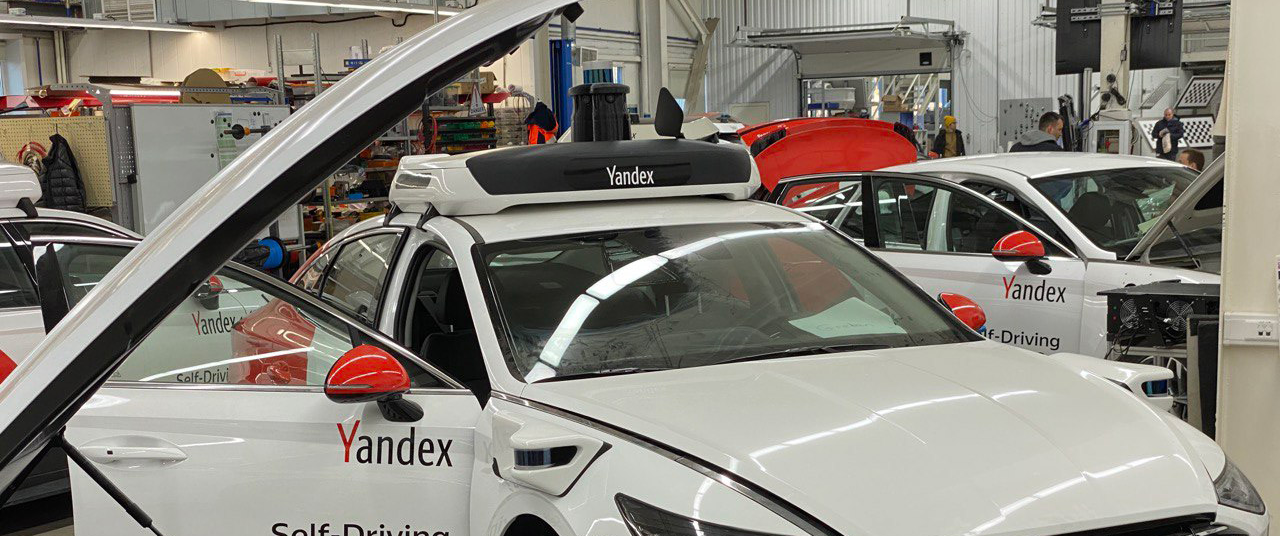
\includegraphics[width=0.4\textwidth]{../source/top.png}
    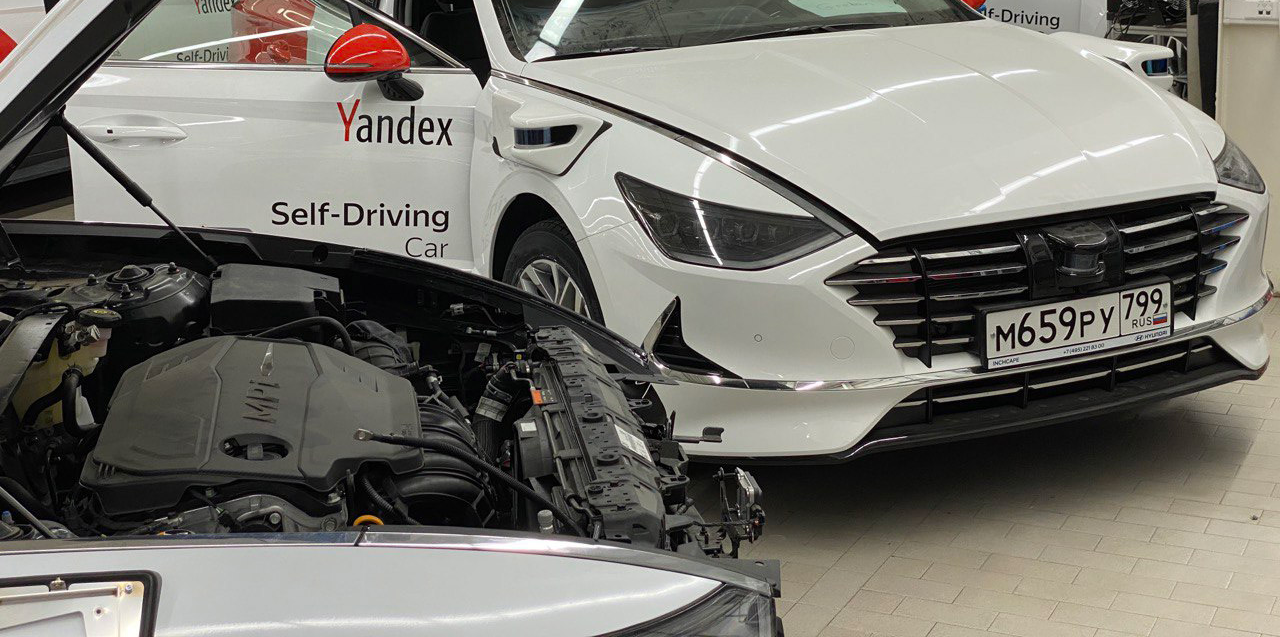
\includegraphics[width=0.5\textwidth]{../source/bttm.png}
    \caption{Изображения для сшивки}
    \label{fig:stitch_images}
\end{figure}

На рисунке \ref{fig:stitch_images} видно, что изображения имеют общую часть, и на основе этой части можно осуществить сшивку.

Посмотрим на несколько способов сшивки изображений:

\begin{lstlisting}[style=cpp_white, caption={Исходный код для сшивки изображений}]
cv::Mat topPart = cv::imread(path + "/lab2/1.jpg");
cv::Mat botPart = cv::imread(path + "/lab2/2.jpg");

int templ_size = 10;
cv::Mat templ = topPart(cv::Rect(0,topPart.rows - templ_size - 1, 
                                        topPart.cols, templ_size));

cv::Mat res;
cv::matchTemplate(botPart, templ, res, cv::TM_CCOEFF);

double min_val, max_val;
cv::Point2i min_loc, max_loc;
cv::minMaxLoc(res, &min_val, & max_val, &min_loc, &max_loc);

cv::Mat image_res = cv::Mat::zeros(topPart.rows + botPart.rows - 
                    max_loc.y - templ_size, topPart.cols, topPart.type());

topPart.copyTo(image_res(cv::Rect(0, 0, topPart.cols, topPart.rows)));

botPart(cv::Rect(0, max_loc.y + templ_size, botPart.cols,
                    botPart.rows - max_loc.y - templ_size)).
                    copyTo(image_res(cv::Rect(0, topPart.rows, botPart.cols, botPart.rows - max_loc.y - templ_size)));

cv::imwrite(path + "/lab2/outputs/image_glues.png", image_res);
cv::imshow("B", image_res);
cv::waitKey(0);
\end{lstlisting}

\pagebreak

\begin{figure}[ht]
    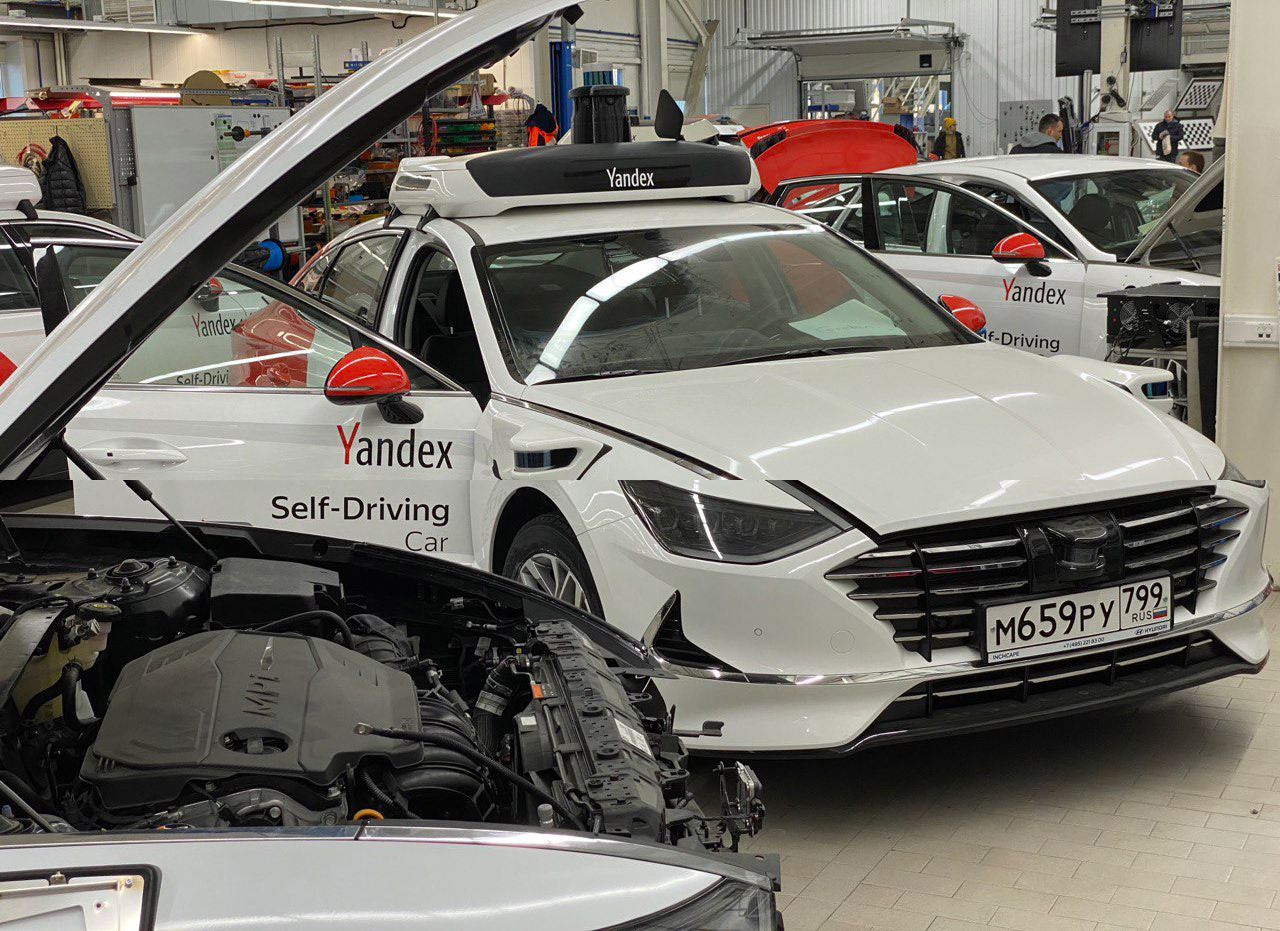
\includegraphics[width=\textwidth]{../outputs/image_glues.png}
    \caption{Сшивка изображений}
    \label{fig:stitched_images}
\end{figure}

Изображение выше имеет выраженную границу сшивки из-за недостаточного исследования матрицы корреляция, что послужило частично неточному определению смежных точек

\begin{lstlisting}[style=cpp_white, caption={Исходный код для сшивки изображений с использованием библиотеки OpenCV}]
cv::Mat topPart = cv::imread(path + "/lab2/source/top.png");
cv::Mat botPart = cv::imread(path + "/lab2/source/bttm.png");
image = cv::imread(path + "/lab2/source/image_cut.png");

cv::Ptr<cv::Stitcher> stitcher = cv::Stitcher::create(cv::Stitcher::SCANS);

std::vector<cv::Mat> imgs;
imgs.push_back(botPart);
imgs.push_back(topPart);

cv::Mat image_stitch;
cv::Stitcher::Status status = stitcher->stitch(imgs, image_stitch);

cv::resize(image_stitch, image_stitch, cv::Size(image.cols, image.rows));

cv::imwrite(path + "/lab2/outputs/image_stitch.png", image_stitch);
cv::imshow("B", image_stitch);
cv::waitKey(0);
\end{lstlisting}

\begin{figure}[ht]
    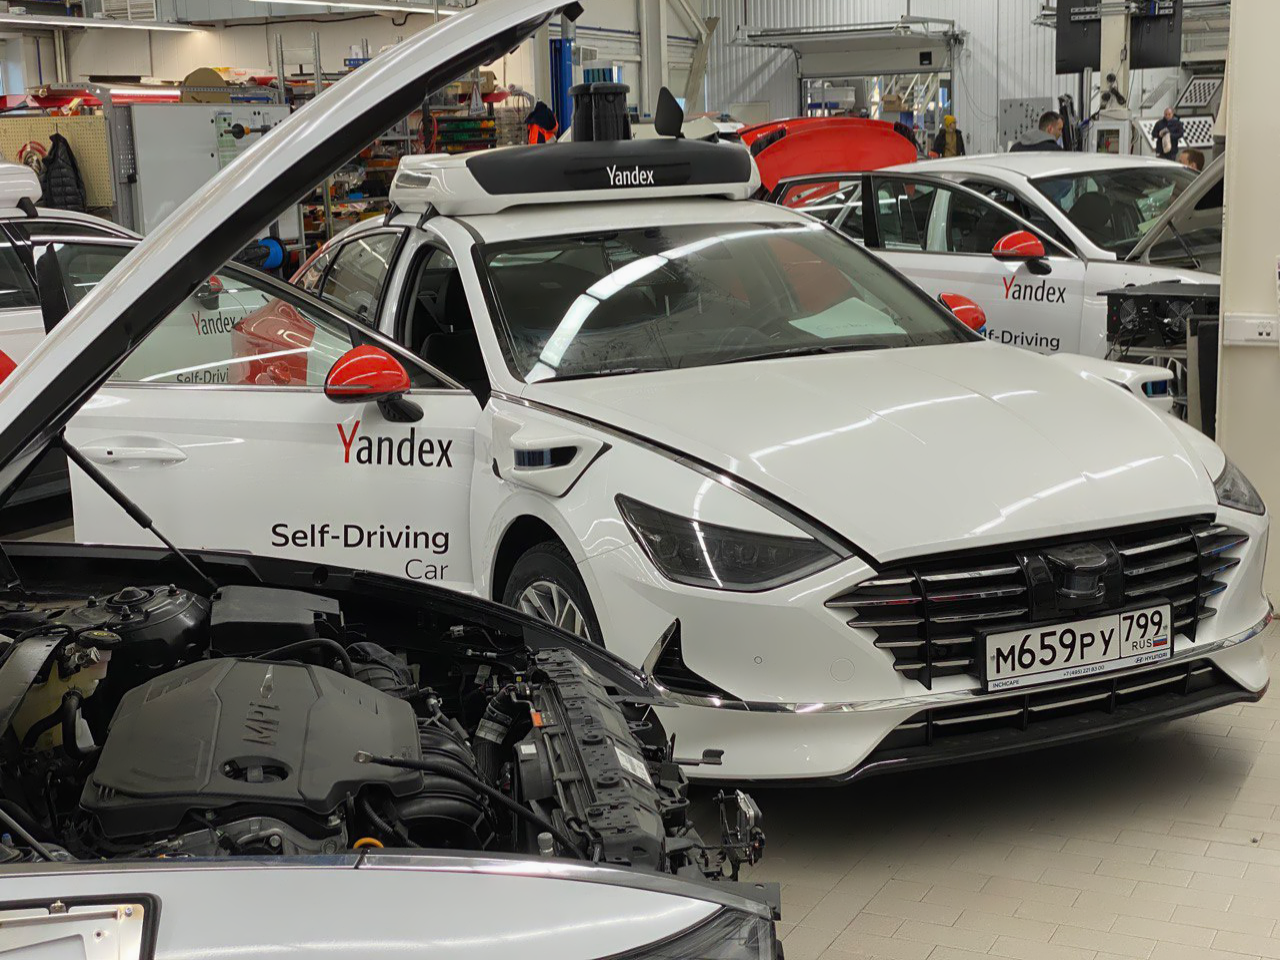
\includegraphics[width=\textwidth]{../outputs/image_stitch.png}
    \caption{Сшивка изображений с использованием библиотеки OpenCV}
    \label{fig:stitched_images_cv}
\end{figure}

Видим, что при использовании каждого из методов изображения были сшиты.

% \pagebreak
\section{Выводы}
В процессе выполнения лабораторной работы мы освоили основные виды отображений и использовали различные геометрические преобразования, попробовали скорректировать оптические искажения. 

Также смогли оценить качество полученных изображений и убедиться, что геометрические преобразования позволяют улучшать их визуальное восприятие

\section{Ответы на вопросы}

\newcounter{question}
\setcounter{question}{0}

\newcommand{\question}[1]{\item[Q\refstepcounter{question}\thequestion.] #1}
\newcommand{\answer}[1]{\item[A\thequestion.] #1}

\begin{itemize}

\question{Каким образом можно выполнить поворот изображения, не используя матрицу поворота?}
\answer{Можно воспользоваться функцией \texttt{cv::rotate()} в библиотеке OpenCV, которая используется как раз для поворота изображения.Она принимает угол вращения в градусах в качестве аргумента. 
По умолчанию размер готового изображения равен размеру исходного изображения, и части повернутого изображения, которые выходят за пределы исходного размера, отсекаются.
Если мы хотим, чтобы повернутое изображение полностью удовлетворяло нашим требованиям, мы можем установить параметр \texttt{expand} в \texttt{True}.}

\question{Какое минимальное количество соответствующих пар точек необходимо задать на исходном и искаженном изображениях, если порядок преобразования $n = 4$?}
\answer{Число минимально необходимых пар точек вычисляется по формуле:

$npair_{min} = ((n+1)\cdot(n+2))/2$, 
где $n$ - порядок преобразования. Следовательно, при $n = 4$ нам потребуется минимум 15 пар точек.}

\question{После геометрического преобразования изображения могут появиться пиксели с неопределенными значениями интенсивности. С чем это связано и как решается данная проблема?}
\answer{При геометрическом преобразовании, когда выполняется трансформация (поворот, масштабирование и т.д.) изображения, пиксели перемещаются и могут попасть в пространство между исходными пикселями. Это приводит к неопределенным значениям интенсивности. 
Для решения этой проблемы используется \textit{интерполяция}. Она позволяет вычислить значения для неопределенных пикселей на основе соседних известных пикселей.}

\end{itemize}

